% generated by GAPDoc2LaTeX from XML source (Frank Luebeck)
\documentclass[a4paper,11pt]{report}

                \usepackage[pdftex]{graphicx} 
                
\usepackage[top=37mm,bottom=37mm,left=27mm,right=27mm]{geometry}
\sloppy
\pagestyle{myheadings}
\usepackage{amssymb}
\usepackage[utf8]{inputenc}
\usepackage{makeidx}
\makeindex
\usepackage{color}
\definecolor{FireBrick}{rgb}{0.5812,0.0074,0.0083}
\definecolor{RoyalBlue}{rgb}{0.0236,0.0894,0.6179}
\definecolor{RoyalGreen}{rgb}{0.0236,0.6179,0.0894}
\definecolor{RoyalRed}{rgb}{0.6179,0.0236,0.0894}
\definecolor{LightBlue}{rgb}{0.8544,0.9511,1.0000}
\definecolor{Black}{rgb}{0.0,0.0,0.0}

\definecolor{linkColor}{rgb}{0.0,0.0,0.554}
\definecolor{citeColor}{rgb}{0.0,0.0,0.554}
\definecolor{fileColor}{rgb}{0.0,0.0,0.554}
\definecolor{urlColor}{rgb}{0.0,0.0,0.554}
\definecolor{promptColor}{rgb}{0.0,0.0,0.589}
\definecolor{brkpromptColor}{rgb}{0.589,0.0,0.0}
\definecolor{gapinputColor}{rgb}{0.589,0.0,0.0}
\definecolor{gapoutputColor}{rgb}{0.0,0.0,0.0}

%%  for a long time these were red and blue by default,
%%  now black, but keep variables to overwrite
\definecolor{FuncColor}{rgb}{0.0,0.0,0.0}
%% strange name because of pdflatex bug:
\definecolor{Chapter }{rgb}{0.0,0.0,0.0}
\definecolor{DarkOlive}{rgb}{0.1047,0.2412,0.0064}


\usepackage{fancyvrb}

\usepackage{mathptmx,helvet}
\usepackage[T1]{fontenc}
\usepackage{textcomp}


\usepackage[
            pdftex=true,
            bookmarks=true,        
            a4paper=true,
            pdftitle={Written with GAPDoc},
            pdfcreator={LaTeX with hyperref package / GAPDoc},
            colorlinks=true,
            backref=page,
            breaklinks=true,
            linkcolor=linkColor,
            citecolor=citeColor,
            filecolor=fileColor,
            urlcolor=urlColor,
            pdfpagemode={UseNone}, 
           ]{hyperref}

\newcommand{\maintitlesize}{\fontsize{50}{55}\selectfont}

% write page numbers to a .pnr log file for online help
\newwrite\pagenrlog
\immediate\openout\pagenrlog =\jobname.pnr
\immediate\write\pagenrlog{PAGENRS := [}
\newcommand{\logpage}[1]{\protect\write\pagenrlog{#1, \thepage,}}
%% were never documented, give conflicts with some additional packages

\newcommand{\GAP}{\textsf{GAP}}

%% nicer description environments, allows long labels
\usepackage{enumitem}
\setdescription{style=nextline}

%% depth of toc
\setcounter{tocdepth}{1}





%% command for ColorPrompt style examples
\newcommand{\gapprompt}[1]{\color{promptColor}{\bfseries #1}}
\newcommand{\gapbrkprompt}[1]{\color{brkpromptColor}{\bfseries #1}}
\newcommand{\gapinput}[1]{\color{gapinputColor}{#1}}


\begin{document}

\logpage{[ 0, 0, 0 ]}
\begin{titlepage}
\mbox{}\vfill

\begin{center}{\maintitlesize \textbf{ idrel \mbox{}}}\\
\vfill

\hypersetup{pdftitle= idrel }
\markright{\scriptsize \mbox{}\hfill  idrel  \hfill\mbox{}}
{\Huge \textbf{ Identities among relations \mbox{}}}\\
\vfill

{\Huge  2.49 \mbox{}}\\[1cm]
{ 2 October 2025 \mbox{}}\\[1cm]
\mbox{}\\[2cm]
{\Large \textbf{ Anne Heyworth\\
 \mbox{}}}\\
{\Large \textbf{ Chris Wensley\\
   \mbox{}}}\\
\hypersetup{pdfauthor= Anne Heyworth\\
 ;  Chris Wensley\\
   }
\end{center}\vfill

\mbox{}\\
{\mbox{}\\
\small \noindent \textbf{ Chris Wensley\\
   }  Email: \href{mailto://cdwensley.maths@btinternet.com} {\texttt{cdwensley.maths@btinternet.com}}\\
  Homepage: \href{https://github.com/cdwensley} {\texttt{https://github.com/cdwensley}}}\\
\end{titlepage}

\newpage\setcounter{page}{2}
{\small 
\section*{Abstract}
\logpage{[ 0, 0, 1 ]}
 \textsf{IdRel} is a \textsf{GAP} package originally implemented in 1999, using the \textsf{GAP} 3 language, when the first author was studying for a Ph.D. in Bangor. 

 This package is designed to compute a minimal set of generators for the module
of the identities among relators of a group presentation. It does this using 
\begin{itemize}
\item  rewriting and logged rewriting: a self\texttt{\symbol{45}}contained
implementation of the Knuth\texttt{\symbol{45}}Bendix process using the monoid
presentation associated to the group presentation; 
\item  monoid polynomials: an implementation of the monoid ring; 
\item  module polynomials: an implementation of the right module over this monoid
generated by the relators. 
\item  Y\texttt{\symbol{45}}sequences: used as a \emph{rewriting} way of representing elements of a free crossed module (products of conjugates
of group relators and inverse relators). 
\end{itemize}
 

 \textsf{IdRel} became an accepted \textsf{GAP} package in May 2015. 

 Bug reports, suggestions and comments are, of course, welcome. Please contact
the last author at \href{mailto://cdwensley.maths@btinternet.com} {\texttt{cdwensley.maths@btinternet.com}} or submit an issue at the GitHub repository \href{https://github.com/gap-packages/idrel/issues/} {\texttt{https://github.com/gap\texttt{\symbol{45}}packages/idrel/issues/}}. \mbox{}}\\[1cm]
{\small 
\section*{Copyright}
\logpage{[ 0, 0, 2 ]}
 {\copyright} 1999\texttt{\symbol{45}}2025 Anne Heyworth and Chris Wensley

 The \textsf{IdRel} package is free software; you can redistribute it and/or modify it under the
terms of the GNU General Public License as published by the Free Software
Foundation; either version 2 of the License, or (at your option) any later
version. \mbox{}}\\[1cm]
{\small 
\section*{Acknowledgements}
\logpage{[ 0, 0, 3 ]}
 This documentation was prepared using the \textsf{GAPDoc} \cite{GAPDoc} and \textsf{AutoDoc} \cite{AutoDoc} packages.

 The procedure used to produce new releases uses the package \textsf{GitHubPagesForGAP} \cite{GitHubPagesForGAP} and the package \textsf{ReleaseTools}.

 \mbox{}}\\[1cm]
\newpage

\def\contentsname{Contents\logpage{[ 0, 0, 4 ]}}

\tableofcontents
\newpage

         
\chapter{\textcolor{Chapter }{Introduction}}\label{intro}
\logpage{[ 1, 0, 0 ]}
\hyperdef{L}{X7DFB63A97E67C0A1}{}
{
  This manual describes the \textsf{IdRel} package for \textsf{GAP} 4.7 for computing the identities among relators of a group presentation using
rewriting, logged rewriting, monoid polynomials, module polynomials and $Y$\texttt{\symbol{45}}sequences. 

 The theoretical background for these computations is contained in Brown and
Huebschumann \cite{BrHu}, Brown and Razak Salleh \cite{BrSa} and is surveyed in the first author's thesis \cite{anne-thesis}. 

 \textsf{IdRel} is primarily designed for the computation of a minimal set of generators for
the module of identities among relators. It also contains functions which
compute logged rewrite systems for group presentations (and complete them
where possible); functions for operations involving elements of monoid rings;
and functions for operations with elements of right modules over monoid rings.
The $Y$\texttt{\symbol{45}}sequences are used as a \emph{rewriting} way of representing elements of a free crossed module (products of conjugates
of group relators and inverse relators). The package is written entirely in \textsf{GAP}4, and requires no compilation. 

 The package is loaded into \textsf{GAP} with the \texttt{LoadPackage} command, and on\texttt{\symbol{45}}line help is available in the usual way. 
\begin{Verbatim}[commandchars=!@|,fontsize=\small,frame=single,label=Example]
  
  !gapprompt@gap>| !gapinput@LoadPackage( "idrel" ); |
  !gapprompt@gap>| !gapinput@?idrel|
  
\end{Verbatim}
 A pdf version of the \textsf{IdRel} manual is available in the \texttt{doc} directory of the home directory of \textsf{IdRel}. The information parameter \texttt{InfoIdRel} has default value \texttt{0}. When raised to a higher value, additional information is printed out. \textsf{IdRel} was originally developed in 1999 using \textsf{GAP}3, partially supported by a University of Wales Research Assistantship for the
first author, Anne Heyworth. 

 If you use \textsf{IdRel} to solve a problem then please send a short email to the second author, to
whom bug reports, suggestions and other comments should also be sent. You may
reference the package by mentioning \cite{HeWe1} and \cite{anne-thesis}. 

 The package may be obtained as a compressed tar file \texttt{idrel\texttt{\symbol{45}}version.number.tar.gz} by ftp from one of the following sites: 
\begin{itemize}
\item  the \textsf{IdRel} GitHub site: \href{https://github.com/gap-packages.github.io/idrel/} {\texttt{https://github.com/gap\texttt{\symbol{45}}packages.github.io/idrel/}}. 
\item  any \textsf{GAP} archive, e.g. \href{https://www.gap-system.org/Packages/packages.html} {\texttt{https://www.gap\texttt{\symbol{45}}system.org/Packages/packages.html}}; 
\end{itemize}
 The package also has a GitHub repository at: \href{https://github.com/gap-packages/idrel/} {\texttt{https://github.com/gap\texttt{\symbol{45}}packages/idrel/}} where issues can be raised. 

 
\section{\textcolor{Chapter }{An illustrative example}}\label{sect-illustration}
\logpage{[ 1, 1, 0 ]}
\hyperdef{L}{X80F39D77788BD099}{}
{
  A typical input for \textsf{IdRel} is an fp\texttt{\symbol{45}}group presentation. This requires a free group \texttt{F} on a set of generators and a set of relators \texttt{R} (words in the free group). The module of identities among relators for this
presentation has as its elements the Peiffer equivalence classes of all
products of conjugates of relators which represent the identity in the free
group. 

 In this package the identities among relators are represented by
Y\texttt{\symbol{45}}sequences, which are lists $[[r_1, u_1],\ldots,[r_k,u_k]]$ where $r_1,\ldots,r_k$ are the group relators or their inverses, and $u_1,\ldots,u_k$ are words in the free group \texttt{F}. A Y\texttt{\symbol{45}}sequence is evaluated in \texttt{F} as the product $(u_1^{-1}r_1u_1)\ldots(u_k^{-1}r_ku_k)$ and is an identity Y\texttt{\symbol{45}}sequence if it evaluates to the
identity in \texttt{F}. An identity Y\texttt{\symbol{45}}sequence represents an identity among the
relators of the group presentation. The main function of the package is to
produce a set of Y\texttt{\symbol{45}}sequences which generate the module of
identites among relators, and further, that this set be minimal in the sense
that every element in it is needed to generate the module. 

 Before starting on the main example, we consider a simpler example
illustrating the use of \textsf{IdRel}. All the functions used are described in detail in this manual. We compute a
reduced set of identities among relators for the presentation of the symmetric
group \texttt{s3 =
F/[f\texttt{\symbol{94}}3,g\texttt{\symbol{94}}2,(fg)\texttt{\symbol{94}}2]}. In the listings below, \texttt{s3{\textunderscore}Ri} is the \texttt{i}\texttt{\symbol{45}}th relator for \texttt{s3}, and \texttt{f1,f2} are the generators $f,g$ of $F$. 

 
\begin{Verbatim}[commandchars=!@|,fontsize=\small,frame=single,label=Example]
  
  !gapprompt@gap>| !gapinput@F := FreeGroup( 2 );; |
  !gapprompt@gap>| !gapinput@f := F.1;;  g := F.2;; |
  !gapprompt@gap>| !gapinput@rels3 := [ f^3, g^2, f*g*f*g ]; |
  [ f1^3, f2^2, (f1*f2)^2 ]
  !gapprompt@gap>| !gapinput@s3 := F/rels3; |
  <fp group on the generators [ f1, f2 ]>
  !gapprompt@gap>| !gapinput@SetName( s3, "s3" );; |
  !gapprompt@gap>| !gapinput@IdentitiesAmongRelators( s3 );|
  [ [ [ -1, <identity ...> ], [ 1, s3_M1 ] ], 
    [ [ -2, <identity ...> ], [ 2, s3_M2 ] ], 
    [ [ -3, <identity ...> ], [ 3, s3_M1*s3_M2 ] ], 
    [ [ 1, <identity ...> ], [ -3, s3_M1 ], [ 2, s3_M3*s3_M4 ], [ 1, s3_M4 ], 
        [ -3, <identity ...> ], [ 2, s3_M3*s3_M4*s3_M3 ], [ 2, s3_M3 ], 
        [ -3, s3_M3 ] ], 
    [ [ 1, <identity ...> ], [ -3, s3_M2 ], [ 2, s3_M3*s3_M4*s3_M3*s3_M2 ], 
        [ 2, s3_M3*s3_M2 ], [ 1, s3_M2 ], [ -3, <identity ...> ], [ 2, s3_M3 ], 
        [ -3, s3_M3 ] ] ]
  
\end{Verbatim}
 If we write $\rho=f^3$, $\sigma=g^2$, $\tau=(fg)^2$ then the first identity becomes $\rho^{-1} \rho^{f}$. Similarly, the second and third identities are the root identities $\sigma^{-1} \sigma^{g}$ and $\tau^{-1} \tau^{fg}$. The fourth identity, which is not a root identity, is obtained by walking
around the Schreier diagram of the presentation, a somewhat truncated
triangular prism. Taking the appropriate conjugate of each face in turn, we
get: 
\[ \rho\ (\tau^{-1})^f\ \sigma^{f^{-1}g^{-1}}\ \rho^{g^{-1}}\ (\tau^{-1})\
\sigma^{f^{-1}g^{-1}f^{-1}}\ \sigma^{f^{-1}}\ (\tau^{-1})^{f^{-1}}\, . \]
 The fifth identity is equivalent to the fourth, as we shall show in section \ref{sect-s3}. 

 In order to form the \emph{module of identities} for \texttt{s3} the identities are transformed into module polynomials. The first is $y_1 = \rho(f-1)$. The second and third are $y_2 = \sigma(g-1)$ and $y_3 = \tau(fg-1)$, while the fourth is $\rho(1+g^{-1}f) + \sigma(1+f^{-1}g^{-1}+f^{-1}g^{-1}f) - \tau(1++f+f^2)$. Note that, in the fourth polynomial, the conjugators are converted to their
normal forms in \texttt{s3}, namely $f^2=f^{-1},\ f^{-1}g^{-1}f=fg,\ g^{-1}f=gf$ and $fg^{-1}f=g$. Generators for this module are returned by the operation \texttt{IdentityYSequences}. 

 
\begin{Verbatim}[commandchars=!@|,fontsize=\small,frame=single,label=Example]
  
  !gapprompt@gap>| !gapinput@idyseq3 := IdentityYSequences( s3 );     |
  [ ( s3_Y1*( -s3_M1), s3_R1*( s3_M1 - <identity ...>) ), 
    ( s3_Y2*( <identity ...>), s3_R2*( s3_M2 - <identity ...>) ), 
    ( s3_Y3*( s3_M1), s3_R3*( s3_M2 - s3_M1) ), 
    ( s3_Y9*( -<identity ...>), s3_R1*( -s3_M2*s3_M1 - s3_M1) + s3_R2*( -s3_M1*s\
  3_M2 - s3_M1 - <identity ...>) + s3_R3*( s3_M3 + s3_M2 + <identity ...>) ) ]
  
\end{Verbatim}
 Further examples are given in chapter \ref{chap-idrels}. 

 An extensive revision has been released with version 2.44. This has
concentrated in the area of log sequences, adding many of the functions
described in sections \ref{sect-s3} and \ref{sect-reducing}. 

 Work on revising Y\texttt{\symbol{45}}sequences is needed, but must wait for
later versions. }

 }

       
\chapter{\textcolor{Chapter }{Rewriting Systems}}\label{chap-rws}
\logpage{[ 2, 0, 0 ]}
\hyperdef{L}{X7CA8FCFD81AA1890}{}
{
  This chapter describes functions to construct rewriting systems for finitely
presented groups which store rewriting information. The main example used
throughout this manual is a presentation of the quaternion group $q8 = F/[a^4, b^4, abab^{-1}, a^2b^2]$. 
\section{\textcolor{Chapter }{Monoid Presentations of FpGroups}}\logpage{[ 2, 1, 0 ]}
\hyperdef{L}{X7875619E84157FC1}{}
{
 

\subsection{\textcolor{Chapter }{FreeRelatorGroup}}
\logpage{[ 2, 1, 1 ]}\nobreak
\hyperdef{L}{X868422B878B0C380}{}
{\noindent\textcolor{FuncColor}{$\triangleright$\enspace\texttt{FreeRelatorGroup({\mdseries\slshape grp})\index{FreeRelatorGroup@\texttt{FreeRelatorGroup}}
\label{FreeRelatorGroup}
}\hfill{\scriptsize (attribute)}}\\
\noindent\textcolor{FuncColor}{$\triangleright$\enspace\texttt{FreeRelatorHomomorphism({\mdseries\slshape grp})\index{FreeRelatorHomomorphism@\texttt{FreeRelatorHomomorphism}}
\label{FreeRelatorHomomorphism}
}\hfill{\scriptsize (attribute)}}\\


 The function \texttt{FreeRelatorGroup} returns a free group on the set of relators of the fp\texttt{\symbol{45}}group \texttt{G}. If \texttt{HasName(G)} is \texttt{true} then a name is automatically assigned to this free group by concatenating \texttt{{\textunderscore}R}. 

 The function \texttt{FreeRelatorHomomorphism} returns the group homomorphism from the free group on the relators to the free
group on the generators of \texttt{G}, mapping each generator to the corresponding word. 

 }

 
\begin{Verbatim}[commandchars=!@|,fontsize=\small,frame=single,label=Example]
  
  !gapprompt@gap>| !gapinput@relq8 := [ f^4, g^4, f*g*f*g^-1, f^2*g^2 ];;|
  !gapprompt@gap>| !gapinput@q8 := F/relq8;;|
  !gapprompt@gap>| !gapinput@SetName( q8, "q8" );;|
  !gapprompt@gap>| !gapinput@q8R := FreeRelatorGroup( q8 ); |
  q8_R
  !gapprompt@gap>| !gapinput@genq8R := GeneratorsOfGroup( q8R );|
  [ q8_R1, q8_R2, q8_R3, q8_R4]
  !gapprompt@gap>| !gapinput@homq8R := FreeRelatorHomomorphism( q8 );|
  [ q8_R1, q8_R2, q8_R3, q8_R4 ] -> [ f1^4, f2^4, f1*f2*f1*f2^-1, f1^2*f2^2 ]
  
\end{Verbatim}
 

\subsection{\textcolor{Chapter }{MonoidPresentationFpGroup}}
\logpage{[ 2, 1, 2 ]}\nobreak
\hyperdef{L}{X7CBE13927DFF4446}{}
{\noindent\textcolor{FuncColor}{$\triangleright$\enspace\texttt{MonoidPresentationFpGroup({\mdseries\slshape grp})\index{MonoidPresentationFpGroup@\texttt{MonoidPresentationFpGroup}}
\label{MonoidPresentationFpGroup}
}\hfill{\scriptsize (attribute)}}\\
\noindent\textcolor{FuncColor}{$\triangleright$\enspace\texttt{ArrangementOfMonoidGenerators({\mdseries\slshape grp})\index{ArrangementOfMonoidGenerators@\texttt{ArrangementOfMonoidGenerators}}
\label{ArrangementOfMonoidGenerators}
}\hfill{\scriptsize (attribute)}}\\
\noindent\textcolor{FuncColor}{$\triangleright$\enspace\texttt{MonoidPresentationLabels({\mdseries\slshape grp})\index{MonoidPresentationLabels@\texttt{MonoidPresentationLabels}}
\label{MonoidPresentationLabels}
}\hfill{\scriptsize (attribute)}}\\
\noindent\textcolor{FuncColor}{$\triangleright$\enspace\texttt{FreeGroupOfPresentation({\mdseries\slshape mon})\index{FreeGroupOfPresentation@\texttt{FreeGroupOfPresentation}}
\label{FreeGroupOfPresentation}
}\hfill{\scriptsize (attribute)}}\\
\noindent\textcolor{FuncColor}{$\triangleright$\enspace\texttt{GroupRelatorsOfPresentation({\mdseries\slshape mon})\index{GroupRelatorsOfPresentation@\texttt{GroupRelatorsOfPresentation}}
\label{GroupRelatorsOfPresentation}
}\hfill{\scriptsize (attribute)}}\\
\noindent\textcolor{FuncColor}{$\triangleright$\enspace\texttt{InverseRelatorsOfPresentation({\mdseries\slshape mon})\index{InverseRelatorsOfPresentation@\texttt{InverseRelatorsOfPresentation}}
\label{InverseRelatorsOfPresentation}
}\hfill{\scriptsize (attribute)}}\\
\noindent\textcolor{FuncColor}{$\triangleright$\enspace\texttt{HomomorphismOfPresentation({\mdseries\slshape mon})\index{HomomorphismOfPresentation@\texttt{HomomorphismOfPresentation}}
\label{HomomorphismOfPresentation}
}\hfill{\scriptsize (attribute)}}\\


 A monoid presentation for a finitely presented group \texttt{G} has two monoid generators $g,G$ for each group generator $g$. The relators of the monoid presentation comprise the group relators, and
relators $gG, Gg$ specifying the inverses. The function \texttt{MonoidPresentationFpGroup} returns the monoid presentation derived in this way from an
fp\texttt{\symbol{45}}presentation. 

 The function \texttt{FreeGroupOfPresentation} returns the free group on the monoid generators. 

 The function \texttt{GroupRelatorsOfPresentation} returns those relators of the monoid which correspond to the relators of the
group. All negative powers in the group relators are converted to positive
powers of the $G$'s. The function \texttt{InverseRelatorsOfPresentation} returns relators which specify the inverse pairs of the monoid generators. 

 The function \texttt{HomomorphismOfPresentation} returns the homomorphism from the free group of the monoid presentation to the
free group of the group presentation. 

 The attribute \texttt{ArrangementOfMonoidGenerators} will be discussed before the second example in the next section. 

 In the example below, the four monoid generators $a,b,A,B$ are named \texttt{q8{\textunderscore}M1, q8{\textunderscore}M2, q8{\textunderscore}M3,
q8{\textunderscore}M4} respectively. }

 
\begin{Verbatim}[commandchars=!@|,fontsize=\small,frame=single,label=Example]
  
  !gapprompt@gap>| !gapinput@mq8 := MonoidPresentationFpGroup( q8 );|
  monoid presentation with group relators 
  [ q8_M1^4, q8_M2^4, q8_M1*q8_M2*q8_M1*q8_M4, q8_M1^2*q8_M2^2 ]
  !gapprompt@gap>| !gapinput@fmq8 := FreeGroupOfPresentation( mq8 ); |
  <free group on the generators [ q8_M1, q8_M2, q8_M3, q8_M4 ]>
  !gapprompt@gap>| !gapinput@genfmq8 := GeneratorsOfGroup( fmq8 );;|
  !gapprompt@gap>| !gapinput@gprels := GroupRelatorsOfPresentation( mq8 ); |
  [ q8_M1^4, q8_M2^4, q8_M1*q8_M2*q8_M1*q8_M4, q8_M1^2*q8_M2^2 ]
  !gapprompt@gap>| !gapinput@invrels := InverseRelatorsOfPresentation( mq8 ); |
  [ q8_M1*q8_M3, q8_M2*q8_M4, q8_M3*q8_M1, q8_M4*q8_M2 ]
  !gapprompt@gap>| !gapinput@hompres := HomomorphismOfPresentation( mq8 ); |
  [ q8_M1, q8_M2, q8_M3, q8_M4 ] -> [ f1, f2, f1^-1, f2^-1 ]
  
\end{Verbatim}
 

\subsection{\textcolor{Chapter }{PrintLnUsingLabels}}
\logpage{[ 2, 1, 3 ]}\nobreak
\hyperdef{L}{X78301362834E55AB}{}
{\noindent\textcolor{FuncColor}{$\triangleright$\enspace\texttt{PrintLnUsingLabels({\mdseries\slshape args})\index{PrintLnUsingLabels@\texttt{PrintLnUsingLabels}}
\label{PrintLnUsingLabels}
}\hfill{\scriptsize (function)}}\\
\noindent\textcolor{FuncColor}{$\triangleright$\enspace\texttt{PrintUsingLabels({\mdseries\slshape args})\index{PrintUsingLabels@\texttt{PrintUsingLabels}}
\label{PrintUsingLabels}
}\hfill{\scriptsize (function)}}\\


 The labels \texttt{q8{\textunderscore}M1, q8{\textunderscore}M2, q8{\textunderscore}M3,
q8{\textunderscore}M4} are rather unhelpful in lengthy output, so it is convenient to use $[a,b,A,B]$ as above. Then the function \texttt{PrintUsingLabels} takes as input a word in the monoid, the generators of the monoid, and a set
of labels for these generators. This function also treats lists of words and
lists of lists in a similar way. The function \texttt{PrintLnUsingLabels} does exactly the same, and then appends a newline. }

 
\begin{Verbatim}[commandchars=!@|,fontsize=\small,frame=single,label=Example]
  
  !gapprompt@gap>| !gapinput@q8labs := [ "a", "b", "A", "B" ];; |
  !gapprompt@gap>| !gapinput@SetMonoidPresentationLabels( q8, q8labs );; |
  !gapprompt@gap>| !gapinput@PrintLnUsingLabels( gprels, genfmq8, q8labs ); |
  [ a^4, b^4, a*b*a*B, a^2*b^2 ]
  
\end{Verbatim}
 

\subsection{\textcolor{Chapter }{InitialRulesOfPresentation}}
\logpage{[ 2, 1, 4 ]}\nobreak
\label{init-rules}
\hyperdef{L}{X7EBBA6A284CC7918}{}
{\noindent\textcolor{FuncColor}{$\triangleright$\enspace\texttt{InitialRulesOfPresentation({\mdseries\slshape mon})\index{InitialRulesOfPresentation@\texttt{InitialRulesOfPresentation}}
\label{InitialRulesOfPresentation}
}\hfill{\scriptsize (function)}}\\


 The initial rules for $mq8$ are the four rules of the form $a^{-1} \to A$; the four rules of the form $aA \to id$; and the four relator rules of the form $a^4 \to id$. }

 
\begin{Verbatim}[commandchars=!@|,fontsize=\small,frame=single,label=Example]
  
  !gapprompt@gap>| !gapinput@q0 := InitialRulesOfPresentation( mq8 );;  |
  !gapprompt@gap>| !gapinput@PrintLnUsingLabels( q0, genfmq8, q8labs );|
  [ [ a^-1, A ], [ b^-1, B ], [ A^-1, a ], [ B^-1, b ], [ a*A, id ], 
  [ b*B, id ], [ A*a, id ], [ B*b, id ], [ a^4, id ], [ a^2*b^2, id ], 
  [ a*b*a*B, id ], [ b^4, id ] ]
  
\end{Verbatim}
 }

 
\section{\textcolor{Chapter }{Rewriting systems for FpGroups}}\logpage{[ 2, 2, 0 ]}
\hyperdef{L}{X7A1F10597D8FC9A9}{}
{
 These functions duplicate the standard Knuth Bendix functions which are
available in the \textsf{GAP} library. There are two reasons for this: (1) these functions were first
written before the standard functions were available; (2) we require logged
versions of the functions, and these are most conveniently extended versions
of the non\texttt{\symbol{45}}logged code. 

\subsection{\textcolor{Chapter }{RewritingSystemFpGroup}}
\logpage{[ 2, 2, 1 ]}\nobreak
\label{rwsfp}
\hyperdef{L}{X858ECE3E807C7363}{}
{\noindent\textcolor{FuncColor}{$\triangleright$\enspace\texttt{RewritingSystemFpGroup({\mdseries\slshape grp})\index{RewritingSystemFpGroup@\texttt{RewritingSystemFpGroup}}
\label{RewritingSystemFpGroup}
}\hfill{\scriptsize (attribute)}}\\


 This function attempts to return a complete rewrite system for the
fp\texttt{\symbol{45}}group \texttt{G} obtained using the group's monoid presentation \texttt{mon}, with a length\texttt{\symbol{45}}lexicographical ordering on the words in \texttt{fgmon}, by applying Knuth\texttt{\symbol{45}}Bendix completion. Such a rewrite
system can be obtained for all finite groups. The rewrite rules are
(partially) ordered, starting with the inverse relators, followed by the rules
which reduce the word length the most. 

 In our \texttt{q8} example there are 20 rewrite rules in the rewriting system \texttt{rws}: \begin{center}
\begin{tabular}{|c|}\hline
 $a^{-1} \to A, \quad b^{-1} \to B, \quad A^{-1} \to a, \quad B^{-1} \to b, $ \\
 $aA \to \rm{id}, \quad bB \to \rm{id}, \quad Aa \to \rm{id}, \quad Bb \to
\rm{id}, $ \\
 $ba \to aB, \quad b^2 \to a^2,\quad bA \to ab, \quad Ab \to aB, \quad A^2 \to
a^2,\quad AB \to ab, $ \\
 $Ba \to ab, \quad BA \to aB, \quad B^2 \to a^2, \quad a^3 \to a, \quad a^2b \to
B, \quad a^2B \to b. $ \\
\hline
\end{tabular}\\[2mm]
\end{center}

 }

 
\begin{Verbatim}[commandchars=!@|,fontsize=\small,frame=single,label=Example]
  
  !gapprompt@gap>| !gapinput@rws := RewritingSystemFpGroup( q8 );;|
  !gapprompt@gap>| !gapinput@Length( rws );|
  20
  !gapprompt@gap>| !gapinput@PrintLnUsingLabels( rws, genfmq8, q8labs );|
  [ [ a^-1, A ], [ b^-1, B ], [ A^-1, a ], [ B^-1, b ], [ a*A, id ], 
  [ b*B, id ], [ A*a, id ], [ B*b, id ], [ b*a, a*B ], [ b^2, a^2 ], 
  [ b*A, a*b ], [ A*b, a*B ], [ A^2, a^2 ], [ A*B, a*b ], [ B*a, a*b ], 
  [ B*A, a*B ], [ B^2, a^2 ], [ a^3, A ], [ a^2*b, B ], [ a^2*B, b ] ]
  
\end{Verbatim}
 The default ordering of the $2n$ monoid generators is $ [g_1^+,g_2^+,\ldots,g_n^+,g_1^-,g_2^-,\ldots,g_n^-] $. In the case of the two\texttt{\symbol{45}}generator abelian group $T = \langle a,b ~|~ [a,b] \rangle$ the Knuth\texttt{\symbol{45}}Bendix process starts to generate infinite sets
of relations such as $\{ab^ma^{-1} \to b^m,~ m \geqslant 1\}$. 

 If, using the \texttt{ArrangementOfMonoidGenerators} function, we specify the alternative ordering $ [g_1^+,g_1^-,g_2^+,g_2^-] $, then a finite set of rules is obtained. 

 
\begin{Verbatim}[commandchars=!@|,fontsize=\small,frame=single,label=Example]
  
  !gapprompt@gap>| !gapinput@T := F/[Comm(f,g)];              |
  <fp group of size infinity on the generators [ f1, f2 ]>
  !gapprompt@gap>| !gapinput@SetName( T, "T" );                   |
  !gapprompt@gap>| !gapinput@SetArrangementOfMonoidGenerators( T, [1,-1,2,-2] );|
  !gapprompt@gap>| !gapinput@Tlabs := [ "x", "X", "y", "Y" ];; |
  !gapprompt@gap>| !gapinput@mT := MonoidPresentationFpGroup( T );              |
  monoid presentation with group relators [ T_M2*T_M4*T_M1*T_M3 ]
  !gapprompt@gap>| !gapinput@fgmT := FreeGroupOfPresentation( mT );; |
  !gapprompt@gap>| !gapinput@genfgmT := GeneratorsOfGroup( fgmT );;|
  !gapprompt@gap>| !gapinput@SetMonoidPresentationLabels( T, Tlabs );; |
  !gapprompt@gap>| !gapinput@rwsT := RewritingSystemFpGroup( T );;|
  !gapprompt@gap>| !gapinput@PrintLnUsingLabels( rwsT, genfgmT, Tlabs );       |
  [ [ x^-1, X ], [ X^-1, x ], [ y^-1, Y ], [ Y^-1, y ], [ x*X, id ], 
  [ X*x, id ], [ y*Y, id ], [ Y*y, id ], [ y*x, x*y ], [ y*X, X*y ], 
  [ Y*x, x*Y ], [ Y*X, X*Y ] ]
  
\end{Verbatim}
 The last four rules show that generators $x$ and $y$ commute. 

\subsection{\textcolor{Chapter }{OnePassReduceWord}}
\logpage{[ 2, 2, 2 ]}\nobreak
\label{one-pass-reduce}
\hyperdef{L}{X83BD6C0A80D88C2C}{}
{\noindent\textcolor{FuncColor}{$\triangleright$\enspace\texttt{OnePassReduceWord({\mdseries\slshape word, rules})\index{OnePassReduceWord@\texttt{OnePassReduceWord}}
\label{OnePassReduceWord}
}\hfill{\scriptsize (operation)}}\\
\noindent\textcolor{FuncColor}{$\triangleright$\enspace\texttt{ReduceWordKB({\mdseries\slshape word, rules})\index{ReduceWordKB@\texttt{ReduceWordKB}}
\label{ReduceWordKB}
}\hfill{\scriptsize (operation)}}\\


 These functions are called by the function \texttt{RewritingSystemFpGroup}. 

 Assuming that \texttt{word} is an element of a free monoid and \texttt{rules} is a list of ordered pairs of such words, the function \texttt{OnePassReduceWord} searches the list of rules until it finds that the
left\texttt{\symbol{45}}hand side of a \texttt{rule} is a \texttt{subword} of \texttt{word}, whereupon it replaces that \texttt{subword} with the right\texttt{\symbol{45}}hand side of the matching rule. The search
is continued from the next \texttt{rule} in \texttt{rules}, but using the new \texttt{word}. When the end of \texttt{rules} is reached, one pass is considered to have been made and the reduced \texttt{word} is returned. If no matches are found then the original \texttt{word} is returned. 

 The function \texttt{ReduceWordKB} repeatedly applies the function \texttt{OnePassReduceWord} until the \texttt{word} remaining contains no left\texttt{\symbol{45}}hand side of a \texttt{rule} as a \texttt{subword}. If \texttt{rules} is a complete rewrite system, then the irreducible \texttt{word} that is returned is unique, otherwise the order of the rules in \texttt{rules} will determine which irreducible word is returned. In our $q8$ example we see that $b^9a^{-9}$ reduces to $ab$. 

 }

 
\begin{Verbatim}[commandchars=!@|,fontsize=\small,frame=single,label=Example]
  
  !gapprompt@gap>| !gapinput@a := genfmq8[1];;  b := genfmq8[2];; |
  !gapprompt@gap>| !gapinput@A := genfmq8[3];;  B := genfmq8[4];; |
  !gapprompt@gap>| !gapinput@w0 := b^9 * a^-9;; |
  !gapprompt@gap>| !gapinput@PrintLnUsingLabels( w0, genfmq8, q8labs ); |
  b^9*a^-9
  !gapprompt@gap>| !gapinput@w1 := OnePassReduceWord( w0, rws );; |
  !gapprompt@gap>| !gapinput@PrintLnUsingLabels( w1, genfmq8, q8labs ); |
  B*b^5*a*b*a^-8
  !gapprompt@gap>| !gapinput@w2 := ReduceWordKB( w0, rws );; |
  !gapprompt@gap>| !gapinput@PrintLnUsingLabels( w2, genfmq8, q8labs ); |
  a*b
  
\end{Verbatim}
 

\subsection{\textcolor{Chapter }{OnePassKB}}
\logpage{[ 2, 2, 3 ]}\nobreak
\label{one-pass-KB}
\hyperdef{L}{X7F0CD1EB7C220D40}{}
{\noindent\textcolor{FuncColor}{$\triangleright$\enspace\texttt{OnePassKB({\mdseries\slshape mon, rules})\index{OnePassKB@\texttt{OnePassKB}}
\label{OnePassKB}
}\hfill{\scriptsize (operation)}}\\


 The function \texttt{OnePassKB} implements the main loop of the Knuth\texttt{\symbol{45}}Bendix completion
algorithm. Rules are compared with each other; all critical pairs are
calculated; and the irreducible critical pairs are orientated with respect to
the length\texttt{\symbol{45}}lexicographical ordering and added to the
rewrite system. 

 The function \texttt{ShorterRule} gives an ordering on rules. Rules $(g_lg_2,id)$ that identify two generators (or one generator with the inverse of another)
come first in the ordering. Otherwise one precedes another if it reduces the
length of a word by a greater amount. 

 One pass of this procedure for our $q8$ example adds $10$ relators to the original $12$. 

 }

 
\begin{Verbatim}[commandchars=!@|,fontsize=\small,frame=single,label=Example]
  
  !gapprompt@gap>| !gapinput@q1 := OnePassKB( mq8, q0 );; |
  !gapprompt@gap>| !gapinput@Length( q1 ); |
  22
  !gapprompt@gap>| !gapinput@PrintLnUsingLabels( q1, genfmq8, q8labs ); |
  [ [ a^-1, A ], [ b^-1, B ], [ A^-1, a ], [ B^-1, b ], [ a*A, id ], 
  [ b*B, id ], [ A*a, id ], [ B*b, id ], [ b^2, a^2 ], [ a^3, A ], 
  [ a^2*b, B ], [ a*b*a, b ], [ a*b^2, A ], [ b*a*B, A ], [ b^3, B ], 
  [ a*b^2, a^3 ], [ b*a*B, a^3 ], [ b^3, a^2*b ], [ a^4, id ], 
  [ a^2*b^2, id ], [ a*b*a*B, id ], [ b^4, id ] ]
  
\end{Verbatim}
 

\subsection{\textcolor{Chapter }{RewriteReduce}}
\logpage{[ 2, 2, 4 ]}\nobreak
\label{rewrite-reduce}
\hyperdef{L}{X844BF013780A746D}{}
{\noindent\textcolor{FuncColor}{$\triangleright$\enspace\texttt{RewriteReduce({\mdseries\slshape mon, rules})\index{RewriteReduce@\texttt{RewriteReduce}}
\label{RewriteReduce}
}\hfill{\scriptsize (operation)}}\\


 The function \texttt{RewriteReduce} will remove unnecessary rules from a rewrite system. A rule is deemed to be
unnecessary if it is implied by the other rules, i.e. if both sides can be
reduced to the same thing by the remaining rules. 

 In the example the $22$ rules in $q1$ are reduced to $13$. 

 }

 
\begin{Verbatim}[commandchars=!@|,fontsize=\small,frame=single,label=Example]
  
  !gapprompt@gap>| !gapinput@q2 := RewriteReduce( mq8, q1 );; |
  !gapprompt@gap>| !gapinput@Length( q2 ); |
  13
  !gapprompt@gap>| !gapinput@PrintLnUsingLabels( q2, genfmq8, q8labs ); |
  [ [ a^-1, A ], [ b^-1, B ], [ A^-1, a ], [ B^-1, b ], [ a*A, id ], 
  [ b*B, id ], [ A*a, id ], [ B*b, id ], [ b^2, a^2 ], [ a^3, A ], 
  [ a^2*b, B ], [ a*b*a, b ], [ b*a*B, A ] ]
  
\end{Verbatim}
 

\subsection{\textcolor{Chapter }{KnuthBendix}}
\logpage{[ 2, 2, 5 ]}\nobreak
\label{Knuth-Bendix}
\hyperdef{L}{X8412C40B7B2DC8E0}{}
{\noindent\textcolor{FuncColor}{$\triangleright$\enspace\texttt{KnuthBendix({\mdseries\slshape mon, rules})\index{KnuthBendix@\texttt{KnuthBendix}}
\label{KnuthBendix}
}\hfill{\scriptsize (operation)}}\\


 The function \texttt{KnuthBendix} implements the Knuth\texttt{\symbol{45}}Bendix algorithm, attempting to
complete a rewrite system with respect to a
length\texttt{\symbol{45}}lexicographic ordering. It calls first \texttt{OnePassKB}, which adds rules, and then (for efficiency) \texttt{RewriteReduce} which removes any unnecessary ones. This procedure is repeated until \texttt{OnePassKB} adds no more rules. It will not always terminate, but for many examples (all
finite groups) it will be successful. The rewrite system returned is complete,
that is: it will rewrite any given word in the free monoid to a unique
irreducible; there is one irreducible for each element of the quotient monoid;
and any two elements of the free monoid which are in the same class will
rewrite to the same irreducible. 

 The function \texttt{ShorterRule} gives an ordering on rules. Rules $(g_lg_2,id)$ that identify two generators (or one generator with the inverse of another)
come first in the ordering. Otherwise one precedes another if it reduces the
length of a word by a greater amount. 

 In the example the function \texttt{KnuthBendix} requires three instances of \texttt{OnePassKB} and \texttt{RewriteReduce} to form the complete rewrite system $rws$ for the group shown above. 

 }

 
\begin{Verbatim}[commandchars=!@|,fontsize=\small,frame=single,label=Example]
  
  !gapprompt@gap>| !gapinput@q3 := KnuthBendix( mq8, q0 );; |
  !gapprompt@gap>| !gapinput@Length( q3 ); |
  20
  !gapprompt@gap>| !gapinput@PrintLnUsingLabels( q3, genfmq8, q8labs ); |
  [ [ a^-1, A ], [ b^-1, B ], [ A^-1, a ], [ B^-1, b ], [ a*A, id ], 
  [ b*B, id ], [ A*a, id ], [ B*b, id ], [ b*a, a*B ], [ b^2, a^2 ], 
  [ b*A, a*b ], [ A*b, a*B ], [ A^2, a^2 ], [ A*B, a*b ], [ B*a, a*b ], 
  [ B*A, a*B ], [ B^2, a^2 ], [ a^3, A ], [ a^2*b, B ], [ a^2*B, b ] ]
  
\end{Verbatim}
 }

 
\section{\textcolor{Chapter }{Enumerating elements}}\logpage{[ 2, 3, 0 ]}
\hyperdef{L}{X83CBF2BE8478A728}{}
{
 

\subsection{\textcolor{Chapter }{ElementsOfMonoidPresentation}}
\logpage{[ 2, 3, 1 ]}\nobreak
\hyperdef{L}{X7EDA50068207339D}{}
{\noindent\textcolor{FuncColor}{$\triangleright$\enspace\texttt{ElementsOfMonoidPresentation({\mdseries\slshape mon})\index{ElementsOfMonoidPresentation@\texttt{ElementsOfMonoidPresentation}}
\label{ElementsOfMonoidPresentation}
}\hfill{\scriptsize (attribute)}}\\


 The function \texttt{ElementsOfMonoidPresentation} returns a list of normal forms for the elements of the group given by the
monoid presentation \texttt{mon}. The normal forms are the least elements in each equivalence class (with
respect to length\texttt{\symbol{45}}lex order).   When \texttt{rules} is a complete rewrite system for \texttt{G} the list returned is a set of normal forms for the group elements. For \texttt{q8} this list is 
\[ [\; {\rm id},\; a^+,\; b^+,\; a^-,\; b^-,\; a^{+2},\; a^+b^+,\; a^+b^-\; ]. \]
 

 }

 
\begin{Verbatim}[commandchars=!@|,fontsize=\small,frame=single,label=Example]
  
  !gapprompt@gap>| !gapinput@elmq8 := ElementsOfMonoidPresentation( q8 );; |
  !gapprompt@gap>| !gapinput@PrintLnUsingLabels( elmq8, genfmq8, q8labs ); |
  [ id, a, b, A, B, a^2, a*b, a*B ]
  
\end{Verbatim}
 }

 }

        
\chapter{\textcolor{Chapter }{Logged Rewriting Systems}}\label{chap-logrws}
\logpage{[ 3, 0, 0 ]}
\hyperdef{L}{X7B8D727485966AF8}{}
{
  A \emph{logged rewrite system} is associated with a group presentation. Each \emph{logged rewrite rule} contains, in addition to the standard rewrite rule, a record or \emph{log component} which expresses the rule in terms of the original relators of the group. We
represent such a rule by a triple \texttt{[ u, [L1,L2,..,Lk], v]}, where \texttt{[u,v]} is a rewrite rule and $L_i = [n_i,w_i]$ where $n_i$ is a group relator and $w_i$ is a word. These three components obey the identity $u = n_1^{w_1} \ldots n_k^{w_k} v$. 

 
\section{\textcolor{Chapter }{Logged Knuth\texttt{\symbol{45}}Bendix Completion}}\logpage{[ 3, 1, 0 ]}
\hyperdef{L}{X797732E87F1FE197}{}
{
 The functions in this section are the logged versions of those in the previous
chapter. 

\subsection{\textcolor{Chapter }{InitialLoggedRulesOfPresentation}}
\logpage{[ 3, 1, 1 ]}\nobreak
\hyperdef{L}{X7F47FE67829B962A}{}
{\noindent\textcolor{FuncColor}{$\triangleright$\enspace\texttt{InitialLoggedRulesOfPresentation({\mdseries\slshape mon})\index{InitialLoggedRulesOfPresentation@\texttt{InitialLoggedRulesOfPresentation}}
\label{InitialLoggedRulesOfPresentation}
}\hfill{\scriptsize (function)}}\\


 The $12$ initial logged rules for $mq8$ correspond to the $12$ initial rules in section \ref{init-rules}. Rules of the form $g^{-1} \to G$ and $gG \to id$ apply to the monoid presentation, but not to the group presentation, so are
given an empty logged component. The remaining four rules, which corresppond
to the relators $r \in [a^4, b^4, abab^{-1}, a^2b^2]$ are given logged components $[r,[\,[n,id]\,], id]$ for $n \in [9..12]$. }

 
\begin{Verbatim}[commandchars=!@|,fontsize=\small,frame=single,label=Example]
  
  !gapprompt@gap>| !gapinput@r0 := InitialLoggedRulesOfPresentation( mq8 );; |
  !gapprompt@gap>| !gapinput@PrintLnUsingLabels( r0, genfmq8, q8labs );|
  [ [ a^-1, [ ], A ], [ b^-1, [ ], B ], [ A^-1, [ ], a ], [ B^-1, 
  [ ], b ], [ a*A, [ ], id ], [ b*B, [ ], id ], [ A*a, [ ], id ], 
  [ B*b, [ ], id ], [ a^4, [ [ 1, id ] ], id ], [ a^2*b^2, [ [ 4, id ] ], id ], 
  [ a*b*a*B, [ [ 3, id ] ], id ], [ b^4, [ [ 2, id ] ], id ] ]
  
\end{Verbatim}
 

\subsection{\textcolor{Chapter }{LoggedOnePassKB}}
\logpage{[ 3, 1, 2 ]}\nobreak
\hyperdef{L}{X80075D5180A8F1A5}{}
{\noindent\textcolor{FuncColor}{$\triangleright$\enspace\texttt{LoggedOnePassKB({\mdseries\slshape grp, loggedrules})\index{LoggedOnePassKB@\texttt{LoggedOnePassKB}}
\label{LoggedOnePassKB}
}\hfill{\scriptsize (operation)}}\\


 Given a logged rewrite system for the group \texttt{grp}, this function finds all the rules that would be added to complete the
rewrite system of \texttt{OnePassKB} in \ref{one-pass-KB}, and also the logs which relate the new rules to the originals. The result of
applying this function to \texttt{loggedrules} is to add new logged rules to the system without changing the monoid it
defines. 

 In the example, we apply one pass of the logged
Knuth\texttt{\symbol{45}}Bendix procedure to the initial set of logged rules. 

 }

 
\begin{Verbatim}[commandchars=!@|,fontsize=\small,frame=single,label=Example]
  
  !gapprompt@gap>| !gapinput@r1 := LoggedOnePassKB( mq8, r0 );;|
  !gapprompt@gap>| !gapinput@Length( r1 );|
  25
  !gapprompt@gap>| !gapinput@PrintLnUsingLabels( r1, genfmq8, q8labs );|
  [ [ a^-1, [ ], A ], [ b^-1, [ ], B ], [ A^-1, [ ], a ], [ B^-1, 
  [ ], b ], [ a*A, [ ], id ], [ b*B, [ ], id ], [ A*a, [ ], id ], 
  [ B*b, [ ], id ], [ b^2, [ [ -4, id ], [ 2, A^2 ] ], a^2 ], 
  [ b^2, [ [ -1, id ], [ 4, A^2 ] ], a^2 ], [ a^3, [ [ 1, id ] ], A ], 
  [ a^3, [ [ 1, a ] ], A ], [ a^2*b, [ [ 4, id ] ], B ], [ a*b*a, 
  [ [ 3, id ] ], b ], [ a*b^2, [ [ 4, a ] ], A ], [ b*a*B, [ 
  [ 3, a ] ], A ], [ b^3, [ [ 2, id ] ], B ], [ b^3, [ [ 2, b ] ], B ], 
  [ a*b^2, [ [ -1, id ], [ 4, A^3 ] ], a^3 ], [ b*a*B, [ [ -1, id ], 
  [ 3, A^3 ] ], a^3 ], [ b^3, [ [ -4, id ], [ 2, B*A^2 ] ], a^2*b ], 
  [ a^4, [ [ 1, id ] ], id ], [ a^2*b^2, [ [ 4, id ] ], id ], 
  [ a*b*a*B, [ [ 3, id ] ], id ], [ b^4, [ [ 2, id ] ], id ] ]
   
\end{Verbatim}
 Note that $r1$ has length $25$, three more than the length $22$ of \texttt{q1} in \ref{one-pass-KB}. This because the three rules $b^2 \to a^2;~ a^3 \to A;~ b^3 \to B$ each appear twice, with alternative logged components. 

 If we write $a,b,A,B$ for \texttt{M1,M2,M3,M4} and label the four original relators as $q=a^4,\ r=b^4,\ s=abaB,\ t=a^2b^2$ then the ninth identity (for example) says that $b^2 = (t^{-1}r^{A^2})a^2$. To verify this, we may expand the right\texttt{\symbol{45}}hand side as
follows: 
\[ (B^2A^2).a^2(b^4)A^2.a^2 ~=~ B^2(A^2a^2)b^4(A^2a^2) ~=~ B^2b^4 ~=~ b^2. \]
 

\subsection{\textcolor{Chapter }{LoggedRewriteReduce}}
\logpage{[ 3, 1, 3 ]}\nobreak
\hyperdef{L}{X7E550C0078AEDC45}{}
{\noindent\textcolor{FuncColor}{$\triangleright$\enspace\texttt{LoggedRewriteReduce({\mdseries\slshape grp, loggedrules})\index{LoggedRewriteReduce@\texttt{LoggedRewriteReduce}}
\label{LoggedRewriteReduce}
}\hfill{\scriptsize (operation)}}\\


 The function \texttt{LoggedRewriteReduce} removes unnecessary rules from a logged rewrite system. It works on the same
principle as \texttt{RewriteReduce} in \ref{rewrite-reduce}. Note that $q2$ nd $r2$ both have length $13$. 

 }

 
\begin{Verbatim}[commandchars=!@|,fontsize=\small,frame=single,label=Example]
  
  !gapprompt@gap>| !gapinput@r2 := LoggedRewriteReduce( mq8, r1 );;|
  !gapprompt@gap>| !gapinput@Length( r2 );|
  13
  !gapprompt@gap>| !gapinput@PrintLnUsingLabels( r2, genfmq8, q8labs );      |
  [ [ a^-1, [ ], A ], [ b^-1, [ ], B ], [ A^-1, [ ], a ], [ B^-1, 
  [ ], b ], [ a*A, [ ], id ], [ b*B, [ ], id ], [ A*a, [ ], id ], 
  [ B*b, [ ], id ], [ b^2, [ [ -4, id ], [ 2, A^2 ] ], a^2 ], 
  [ a^3, [ [ 1, id ] ], A ], [ a^2*b, [ [ 4, id ] ], B ], [ a*b*a, 
  [ [ 3, id ] ], b ], [ b*a*B, [ [ 3, a ] ], A ] ]
  
\end{Verbatim}
 

\subsection{\textcolor{Chapter }{LoggedKnuthBendix}}
\logpage{[ 3, 1, 4 ]}\nobreak
\hyperdef{L}{X87D1E3A578AAAFCB}{}
{\noindent\textcolor{FuncColor}{$\triangleright$\enspace\texttt{LoggedKnuthBendix({\mdseries\slshape grp, loggedrules})\index{LoggedKnuthBendix@\texttt{LoggedKnuthBendix}}
\label{LoggedKnuthBendix}
}\hfill{\scriptsize (operation)}}\\


 The function \texttt{LoggedKnuthBendix} repeatedly applies functions \texttt{LoggedOnePassKB} and \texttt{LoggedRewriteReduce} until no new rules are added and no unnecessary ones are included. The output
is a reduced complete logged rewrite system. 

 As a further example, consider the ninth rule in \texttt{r3} which shows how $ba$ reduces to $aB$. For this rule \texttt{[u,L,v]} we will verify that $u = n_1^{w_1}n_2^{w_2}n_3^{w_3} v$, as in the introduction to this chapter. The rule is: 
\[ [ ba, [ [-11,id], [12,BA] ], aB ]. \]
 The relators are $-11 \equiv s^{-1} = bABA$ and $12 \equiv t = a^2b^2$. These are conjugated by the identity and $BA$ respectively. So the second and third parts of the rule expand to: 
\[ (bABA)(ab(aabb)BA)aB ~=~ bAB(Aa)baab(bB)(Aa)B ~=~ bA(Bb)aa(bB) ~=~ b(Aa)a ~=~
ba, \]
 the first part of the rule. 

 }

 
\begin{Verbatim}[commandchars=!@|,fontsize=\small,frame=single,label=Example]
  
  !gapprompt@gap>| !gapinput@r3 := LoggedKnuthBendix( mq8, r0 );;|
  !gapprompt@gap>| !gapinput@Length( r3 );|
  20
  !gapprompt@gap>| !gapinput@PrintLnUsingLabels( r3, genfmq8, q8labs );|
  [ [ a^-1, [ ], A ], [ b^-1, [ ], B ], [ A^-1, [ ], a ], [ B^-1, 
  [ ], b ], [ a*A, [ ], id ], [ b*B, [ ], id ], [ A*a, [ ], id ], 
  [ B*b, [ ], id ], [ b*a, [ [ -3, id ], [ 4, B*A ] ], a*B ], 
  [ b^2, [ [ -4, id ], [ 2, A^2 ] ], a^2 ], [ b*A, [ [ -3, id ] ], a*b ], 
  [ A*b, [ [ -1, id ], [ 4, A ] ], a*B ], [ A^2, [ [ -1, id ] ], a^2 ], 
  [ A*B, [ [ -4, a ] ], a*b ], [ B*a, [ [ -4, id ], [ 3, A ] ], a*b ], 
  [ B*A, [ [ -3, a*b ] ], a*B ], [ B^2, [ [ -4, id ] ], a^2 ], 
  [ a^3, [ [ 1, id ] ], A ], [ a^2*b, [ [ 4, id ] ], B ], [ a^2*B, 
  [ [ -4, A^2 ], [ 1, id ] ], b ] ]
  
\end{Verbatim}
 

\subsection{\textcolor{Chapter }{LoggedRewritingSystemFpGroup}}
\logpage{[ 3, 1, 5 ]}\nobreak
\hyperdef{L}{X8652CEEF7802DA46}{}
{\noindent\textcolor{FuncColor}{$\triangleright$\enspace\texttt{LoggedRewritingSystemFpGroup({\mdseries\slshape grp})\index{LoggedRewritingSystemFpGroup@\texttt{LoggedRewritingSystemFpGroup}}
\label{LoggedRewritingSystemFpGroup}
}\hfill{\scriptsize (attribute)}}\\


 Given a group presentation, the function \texttt{LoggedRewritingSystemFpGroup} determines a logged rewrite system based on the relators. The initial logged
rewrite system associated with a group presentation consists of two types of
rule. These are logged versions of the two types of rule in the monoid
presentation. Corresponding to the j\texttt{\symbol{45}}th relator \texttt{rel} of the group there is a logged rule \texttt{[rel,[[j,id]],id]}. For each inverse relator there is a logged rule \texttt{[ gen*inv, [], id ]}. The function then attempts a completion of the logged rewrite system. The
rules in the final system are partially ordered by the function \texttt{ShorterLoggedRule}. 

 }

 
\begin{Verbatim}[commandchars=!@|,fontsize=\small,frame=single,label=Example]
  
  !gapprompt@gap>| !gapinput@lrws := LoggedRewritingSystemFpGroup( q8 );;|
  !gapprompt@gap>| !gapinput@PrintLnUsingLabels( lrws, genfgmon, q8labs );|
  [ [ a^-1, [ ], A ], [ b^-1, [ ], B ], [ A^-1, [ ], a ], [ B^-1, 
  [ ], b ], [ a*A, [ ], id ], [ b*B, [ ], id ], [ A*a, [ ], id ], 
  [ B*b, [ ], id ], [ b*a, [ [ -3, id ], [ 4, B*A ] ], a*B ], 
  [ b^2, [ [ -4, id ], [ 2, A^2 ] ], a^2 ], [ b*A, [ [ -3, id ] ], a*b ], 
  [ A*b, [ [ -1, id ], [ 4, A ] ], a*B ], [ A^2, [ [ -1, id ] ], a^2 ], 
  [ A*B, [ [ -4, a ] ], a*b ], [ B*a, [ [ -4, id ], [ 3, A ] ], a*b ], 
  [ B*A, [ [ -3, a*b ] ], a*B ], [ B^2, [ [ -4, id ] ], a^2 ], 
  [ a^3, [ [ 1, id ] ], A ], [ a^2*b, [ [ 4, id ] ], B ], [ a^2*B, 
  [ [ -4, A^2 ], [ 1, id ] ], b ] ]
  !gapprompt@gap>| !gapinput@Length( lrws );|
  16
  
\end{Verbatim}
 

 Consider now the two\texttt{\symbol{45}}generator abelian group $T$ considered in the previous chapter (\ref{rwsfp}). Using the alternative ordering on the monoid generators, \texttt{[ T{\textunderscore}M1}$=a$, \texttt{T{\textunderscore}M2}$=A$, \texttt{T{\textunderscore}M3}$=b$, \texttt{T{\textunderscore}M4}$=B$ \texttt{]}, we obtain the following set of $8$ logged rules. The last of these may be checked as follows: 
\[ (ba(BAba)AB)ab ~=~ ba(B(A(b(aA)B)a)b) \]
 and is a logged version of the rule $ba \to ab$. 

 
\begin{Verbatim}[commandchars=!@|,fontsize=\small,frame=single,label=Example]
  
  !gapprompt@gap>| !gapinput@lrwsT := LoggedRewritingSystemFpGroup( T );;|
  !gapprompt@gap>| !gapinput@PrintLnUsingLabels( lrwsT, genfgmonT, Tlabs );|
  [ [ x^-1, [ ], X ], [ X^-1, [ ], x ], [ y^-1, [ ], Y ], [ Y^-1, 
  [ ], y ], [ x*X, [ ], id ], [ X*x, [ ], id ], [ y*Y, [ ], id ], 
  [ Y*y, [ ], id ], [ y*x, [ [ -1, X*Y ] ], x*y ], [ y*X, [ [ 1, Y ] ], X*y ], 
  [ Y*x, [ [ 1, X ] ], x*Y ], [ Y*X, [ [ -1, id ] ], X*Y ] ]
  
\end{Verbatim}
 }

 
\section{\textcolor{Chapter }{Logged reduction of a word}}\logpage{[ 3, 2, 0 ]}
\hyperdef{L}{X831A93087918AA5D}{}
{
 

\subsection{\textcolor{Chapter }{LoggedReduceWordKB}}
\logpage{[ 3, 2, 1 ]}\nobreak
\hyperdef{L}{X7C5094AF784A8BA7}{}
{\noindent\textcolor{FuncColor}{$\triangleright$\enspace\texttt{LoggedReduceWordKB({\mdseries\slshape word, loggedrules})\index{LoggedReduceWordKB@\texttt{LoggedReduceWordKB}}
\label{LoggedReduceWordKB}
}\hfill{\scriptsize (operation)}}\\
\noindent\textcolor{FuncColor}{$\triangleright$\enspace\texttt{LoggedOnePassReduceWord({\mdseries\slshape word, loggedrules})\index{LoggedOnePassReduceWord@\texttt{LoggedOnePassReduceWord}}
\label{LoggedOnePassReduceWord}
}\hfill{\scriptsize (operation)}}\\
\noindent\textcolor{FuncColor}{$\triangleright$\enspace\texttt{ShorterLoggedRule({\mdseries\slshape logrule1, logrule2})\index{ShorterLoggedRule@\texttt{ShorterLoggedRule}}
\label{ShorterLoggedRule}
}\hfill{\scriptsize (operation)}}\\


 Given a word and a logged rewrite system, the function \texttt{LoggedOnePassReduceWord} makes one reduction pass of the word (possibly involving several reductions)
(as does \texttt{OnePassReduceWord} in \ref{one-pass-reduce}) and records this, using the log part of the rule(s) used and the position in
the original word of the replaced part. 

 The function \texttt{LoggedReduceWordKB} repeatedly applies \texttt{OnePassLoggedReduceWord} until the word can no longer be reduced. Each step of the reduction is logged,
showing how the original word can be expressed in terms of the original
relators and the irreducible word. When \texttt{loggedrules} is complete the reduced word is a unique normal form for that group element.
The log of the reduction depends on the order in which the rules are applied. 

 The function \texttt{ShorterLoggedrule} decides whether one logged rule is better than another, using the same
criteria as \texttt{ShorterRule} in \ref{one-pass-KB}. In the example we perform logged reductions of $w_0 = a^9b^{-9}$ corresponding to the ordinary reductions performed in the previous chapter
(section \ref{one-pass-reduce}). 

 In order to clarify the following output, note that, in the log below, $b^9a^{-9}$ reduces to $Bb^5aba^{-8}$ in \texttt{lw1}, just as in section \ref{one-pass-reduce}. This may be checked by cancelling terms in: 
\[ (b^2A^2)(a^2.b^4.A^2)(a^2b^6.bABA.b^6A^2)(a^2b^2)Bb^5aba^{-8} ~=~ b^9a^9. \]
 The corresponding expansion of \texttt{lw2} is too lengthy to include here. (It's hard to believe that the logged part of
this identity is the simplest possible. Further investigation is needed to
determine whether or not this logged part can be simplified.) 

 }

 
\begin{Verbatim}[commandchars=!@|,fontsize=\small,frame=single,label=Example]
  
  !gapprompt@gap>| !gapinput@PrintLnUsingLabels( w0, genfmq8, q8labs ); |
  b^9*a^-9
  !gapprompt@gap>| !gapinput@lw1 := LoggedOnePassReduceWord( w0, lrws );;|
  !gapprompt@gap>| !gapinput@PrintLnUsingLabels( lw1, genfmq8, q8labs );  |
  [ [ [ -4, id ], [ 2, A^2 ], [ -3, b^-6*a^-2 ], [ 4, id ] ], 
  B*b^5*a*b*a^-8 ]
  !gapprompt@gap>| !gapinput@lw2 := LoggedReduceWordKB( w0, lrws );; |
  !gapprompt@gap>| !gapinput@PrintLnUsingLabels( lw2, genfmq8, q8labs );|
  [ [ [ -4, id ], [ 2, A^2 ], [ -3, b^-6*a^-2 ], [ 4, id ], [ -3, b^-3 ], 
  [ 4, B*A*b^-3 ], [ -4, id ], [ 2, A^2 ], [ -3, B^-1*a^-1*b^-1*a^-2 ], 
  [ -4, a^-1*b^-1*a^-2 ], [ 3, A*a^-1*b^-1*a^-2 ], [ 4, id ], 
  [ -4, a^-2*B^-1 ], [ 2, A^2*a^-2*B^-1 ], [ -4, id ], [ 3, A ], 
  [ 1, b^-1*a^-1 ], [ -3, a^-1 ], [ -1, b^-1*a^-2 ], [ 4, id ], 
  [ -3, a*b ], [ -3, a*b*a^-1 ], [ -4, A^2 ], [ 1, id ], [ -3, id ] ], a*b ]
  
\end{Verbatim}
 }

 }

        
\chapter{\textcolor{Chapter }{Monoid Polynomials}}\label{chap-monpoly}
\logpage{[ 4, 0, 0 ]}
\hyperdef{L}{X83B25026816C87CE}{}
{
  This chapter describes functions to compute with elements of a free
noncommutative algebra. The elements of the algebra are sums of rational
multiples of words in a free monoid. These are called \emph{monoid polynomials}, and are stored as lists of pairs \texttt{[coefficient, word]}. 
\section{\textcolor{Chapter }{Construction of monoid polynomials}}\logpage{[ 4, 1, 0 ]}
\hyperdef{L}{X7E8CE44085FE959D}{}
{
 

\subsection{\textcolor{Chapter }{MonoidPolyFromCoeffsWords}}
\logpage{[ 4, 1, 1 ]}\nobreak
\hyperdef{L}{X7DE231F282DB8660}{}
{\noindent\textcolor{FuncColor}{$\triangleright$\enspace\texttt{MonoidPolyFromCoeffsWords({\mdseries\slshape coeffs, words})\index{MonoidPolyFromCoeffsWords@\texttt{MonoidPolyFromCoeffsWords}}
\label{MonoidPolyFromCoeffsWords}
}\hfill{\scriptsize (operation)}}\\
\noindent\textcolor{FuncColor}{$\triangleright$\enspace\texttt{MonoidPoly({\mdseries\slshape terms})\index{MonoidPoly@\texttt{MonoidPoly}}
\label{MonoidPoly}
}\hfill{\scriptsize (operation)}}\\
\noindent\textcolor{FuncColor}{$\triangleright$\enspace\texttt{ZeroMonoidPoly({\mdseries\slshape F})\index{ZeroMonoidPoly@\texttt{ZeroMonoidPoly}}
\label{ZeroMonoidPoly}
}\hfill{\scriptsize (operation)}}\\


 There are two ways to input a monoid polynomial: by listing the coefficients
and then the words; or by listing the terms as a list of pairs \texttt{[coefficient, word]}. If a word occurs more than once in the input list, the coefficients will be
added so that the terms of the monoid polynomial recorded do not contain any
duplicates. The zero monoid polynomial is the polynomial with no terms. 

 }

 
\begin{Verbatim}[commandchars=@|A,fontsize=\small,frame=single,label=Example]
  
  @gapprompt|gap>A @gapinput|relq8 := RelatorsOfFpGroup( q8 ); A
  [ f1^4, f2^4, f1*f2*f1*f2^-1, f1^2*f2^2 ]
  @gapprompt|gap>A @gapinput|freeq8 := FreeGroupOfFpGroup( q8 );; A
  @gapprompt|gap>A @gapinput|gens := GeneratorsOfGroup( freeq8 );;A
  @gapprompt|gap>A @gapinput|famfree := ElementsFamily( FamilyObj( freeq8 ) );; A
  @gapprompt|gap>A @gapinput|famfree!.monoidPolyFam := MonoidPolyFam;; A
  @gapprompt|gap>A @gapinput|cg := [6,7];; A
  @gapprompt|gap>A @gapinput|pg := MonoidPolyFromCoeffsWords( cg, gens );; A
  @gapprompt|gap>A @gapinput|Print( pg, "\n" ); A
  7*f2 + 6*f1
  @gapprompt|gap>A @gapinput|cr := [3,4,-5,-2];;A
  @gapprompt|gap>A @gapinput|pr := MonoidPolyFromCoeffsWords( cr, relq8 );; A
  @gapprompt|gap>A @gapinput|Print( pr, "\n" );A
  4*f2^4 - 5*f1*f2*f1*f2^-1 - 2*f1^2*f2^2 + 3*f1^4
  @gapprompt|gap>A @gapinput|Print( ZeroMonoidPoly( freeq8 ), "\n" );A
  zero monpoly 
  
\end{Verbatim}
 }

 
\section{\textcolor{Chapter }{Components of a polynomial}}\logpage{[ 4, 2, 0 ]}
\hyperdef{L}{X84B1F4CC79983A94}{}
{
 

\subsection{\textcolor{Chapter }{Terms (for monoid polynomials)}}
\logpage{[ 4, 2, 1 ]}\nobreak
\hyperdef{L}{X810C636178EA42D0}{}
{\noindent\textcolor{FuncColor}{$\triangleright$\enspace\texttt{Terms({\mdseries\slshape poly})\index{Terms@\texttt{Terms}!for monoid polynomials}
\label{Terms:for monoid polynomials}
}\hfill{\scriptsize (attribute)}}\\
\noindent\textcolor{FuncColor}{$\triangleright$\enspace\texttt{Coeffs({\mdseries\slshape poly})\index{Coeffs@\texttt{Coeffs}}
\label{Coeffs}
}\hfill{\scriptsize (attribute)}}\\
\noindent\textcolor{FuncColor}{$\triangleright$\enspace\texttt{Words({\mdseries\slshape poly})\index{Words@\texttt{Words}}
\label{Words}
}\hfill{\scriptsize (attribute)}}\\
\noindent\textcolor{FuncColor}{$\triangleright$\enspace\texttt{LeadTerm({\mdseries\slshape poly})\index{LeadTerm@\texttt{LeadTerm}!for monoid polynomials}
\label{LeadTerm:for monoid polynomials}
}\hfill{\scriptsize (attribute)}}\\
\noindent\textcolor{FuncColor}{$\triangleright$\enspace\texttt{LeadCoeffMonoidPoly({\mdseries\slshape poly})\index{LeadCoeffMonoidPoly@\texttt{LeadCoeffMonoidPoly}}
\label{LeadCoeffMonoidPoly}
}\hfill{\scriptsize (attribute)}}\\


 The function \texttt{Terms} returns the terms of a polynomial as a list of pairs of the form \texttt{[word, coefficient]}. The function \texttt{Coeffs} returns the coefficients of a polynomial as a list, and the function \texttt{Words} returns the words of a polynomial as a list. The function \texttt{LeadTerm} returns the term of the polynomial whose word component is the largest with
respect to the length\texttt{\symbol{45}}lexicographical ordering. The
function \texttt{LeadCoeffMonoidPoly} returns the coefficient of the leading term of a polynomial. 

 }

 
\begin{Verbatim}[commandchars=!@|,fontsize=\small,frame=single,label=Example]
  
  !gapprompt@gap>| !gapinput@Coeffs( pr );|
  [ 4, -5, -2, 3 ]
  !gapprompt@gap>| !gapinput@Terms( pr );|
  [ [ 4, f2^4 ], [ -5, f1*f2*f1*f2^-1 ], [ -2, f1^2*f2^2 ], [ 3, f1^4 ] ]
  !gapprompt@gap>| !gapinput@Words( pr );|
  [ f2^4, f1*f2*f1*f2^-1, f1^2*f2^2, f1^4 ]
  !gapprompt@gap>| !gapinput@LeadTerm( pr );|
  [ 4, f2^4 ]
  !gapprompt@gap>| !gapinput@LeadCoeffMonoidPoly( pr );|
  4
  
\end{Verbatim}
 

\subsection{\textcolor{Chapter }{Monic}}
\logpage{[ 4, 2, 2 ]}\nobreak
\hyperdef{L}{X85C78946877C1FF5}{}
{\noindent\textcolor{FuncColor}{$\triangleright$\enspace\texttt{Monic({\mdseries\slshape poly})\index{Monic@\texttt{Monic}}
\label{Monic}
}\hfill{\scriptsize (operation)}}\\


 A monoid polynomial is called \emph{monic} if the coefficient of its leading polynomial is one. The function \texttt{Monic} converts a polynomial into a monic polynomial by dividing all the coefficients
by the leading coefficient. 

 }

 
\begin{Verbatim}[commandchars=!@|,fontsize=\small,frame=single,label=Example]
  
  !gapprompt@gap>| !gapinput@mpr := Monic( pr );; |
  !gapprompt@gap>| !gapinput@Print( mpr, "\n" ); |
   f2^4 - 5/4*f1*f2*f1*f2^-1 - 1/2*f1^2*f2^2 + 3/4*f1^4
  
\end{Verbatim}
 

\subsection{\textcolor{Chapter }{AddTermMonoidPoly}}
\logpage{[ 4, 2, 3 ]}\nobreak
\hyperdef{L}{X82E04F1086DAAA43}{}
{\noindent\textcolor{FuncColor}{$\triangleright$\enspace\texttt{AddTermMonoidPoly({\mdseries\slshape poly, coeff, word})\index{AddTermMonoidPoly@\texttt{AddTermMonoidPoly}}
\label{AddTermMonoidPoly}
}\hfill{\scriptsize (operation)}}\\


 The function \texttt{AddTermMonoidPoly} adds a new term, given by its coeffiecient and word, to an existing
polynomial. 

 }

 
\begin{Verbatim}[commandchars=!@|,fontsize=\small,frame=single,label=Example]
  
  !gapprompt@gap>| !gapinput@w := gens[1]^gens[2]; |
  f2^-1*f1*f2
  !gapprompt@gap>| !gapinput@cw := 3/4;;  |
  !gapprompt@gap>| !gapinput@wpg := AddTermMonoidPoly( pg, cw, w );;|
  !gapprompt@gap>| !gapinput@Print( wpg, "\n" );|
  3/4*f2^-1*f1*f2 + 7*f2 + 6*f1
  
\end{Verbatim}
 }

 
\section{\textcolor{Chapter }{Monoid Polynomial Operations}}\logpage{[ 4, 3, 0 ]}
\hyperdef{L}{X832341AB7A04BA45}{}
{
 \index{=,+,* for monoid polynomials} Tests for equality and arithmetic operations are performed in the usual way. 

 The operation \texttt{poly1 = poly2} returns \texttt{true} if the monoid polynomials have the same terms, and \texttt{false} otherwise. Multiplication of a monoid polynomial (on the left or right) by a
coefficient; the addition or subtraction of two monoid polynomials;
multiplication (on the right) of a monoid polynomial by a word; and
multiplication of two monoid polynomials; are all implemented. 

 
\begin{Verbatim}[commandchars=!@|,fontsize=\small,frame=single,label=Example]
  
  !gapprompt@gap>| !gapinput@[ pg = pg, pg = pr ]; |
  [ true, false ]
  !gapprompt@gap>| !gapinput@prcw := pr * cw;;|
  !gapprompt@gap>| !gapinput@Print( prcw, "\n" ); |
  3*f2^4 - 15/4*f1*f2*f1*f2^-1 - 3/2*f1^2*f2^2 + 9/4*f1^4
  !gapprompt@gap>| !gapinput@cwpr := cw * pr;;|
  !gapprompt@gap>| !gapinput@Print( cwpr, "\n" ); |
  3*f2^4 - 15/4*f1*f2*f1*f2^-1 - 3/2*f1^2*f2^2 + 9/4*f1^4
  !gapprompt@gap>| !gapinput@[ pr = prcw, prcw = cwpr ];|
  [ false, true ]
  !gapprompt@gap>| !gapinput@Print( pg + pr, "\n" );|
  4*f2^4 - 5*f1*f2*f1*f2^-1 - 2*f1^2*f2^2 + 3*f1^4 + 7*f2 + 6*f1
  !gapprompt@gap>| !gapinput@Print( pg - pr, "\n" );|
   - 4*f2^4 + 5*f1*f2*f1*f2^-1 + 2*f1^2*f2^2 - 3*f1^4 + 7*f2 + 6*f1
  !gapprompt@gap>| !gapinput@Print( pg * w, "\n" );|
  6*f1*f2^-1*f1*f2 + 7*f1*f2
  !gapprompt@gap>| !gapinput@Print( pg * pr, "\n" );|
  28*f2^5 - 35*(f2*f1)^2*f2^-1 - 14*f2*f1^2*f2^2 + 21*f2*f1^4 + 24*f1*f2^4 - 
  30*f1^2*f2*f1*f2^-1 - 12*f1^3*f2^2 + 18*f1^5
  
\end{Verbatim}
 

\subsection{\textcolor{Chapter }{Length (for monoid polynomials)}}
\logpage{[ 4, 3, 1 ]}\nobreak
\hyperdef{L}{X86C2C49080691991}{}
{\noindent\textcolor{FuncColor}{$\triangleright$\enspace\texttt{Length({\mdseries\slshape poly})\index{Length@\texttt{Length}!for monoid polynomials}
\label{Length:for monoid polynomials}
}\hfill{\scriptsize (method)}}\\


 This function returns the number of distinct terms in the monoid polynomial. 

 The boolean function \texttt{poly1 {\textgreater} poly2} returns \texttt{true} if the first polynomial has more terms than the second. If the polynomials are
the same length it will compare their leading terms. If the leading word of
the first is lengthlexicographically greater than the leading word of the
second, or if the words are equal but the coefficient of the first is greater
than the coefficient of the second then true is returned. If the leading terms
are equal then the next terms are compared in the same way. If all terms are
the same then \texttt{false} is returned. 

 }

 
\begin{Verbatim}[commandchars=!@|,fontsize=\small,frame=single,label=Example]
  
  !gapprompt@gap>| !gapinput@Length( pr );|
  4
  !gapprompt@gap>| !gapinput@[ pr > 3*pr, pr > pg ];|
  [ false, true ] 
  
\end{Verbatim}
 }

 
\section{\textcolor{Chapter }{Reduction of a Monoid Polynomial}}\logpage{[ 4, 4, 0 ]}
\hyperdef{L}{X7A80EA5C7AEA68B1}{}
{
 

\subsection{\textcolor{Chapter }{ReduceMonoidPoly}}
\logpage{[ 4, 4, 1 ]}\nobreak
\label{reduce-monoid-poly}
\hyperdef{L}{X7979DE308676398D}{}
{\noindent\textcolor{FuncColor}{$\triangleright$\enspace\texttt{ReduceMonoidPoly({\mdseries\slshape poly, rules})\index{ReduceMonoidPoly@\texttt{ReduceMonoidPoly}}
\label{ReduceMonoidPoly}
}\hfill{\scriptsize (operation)}}\\


 Recall that the words of a monoid polynomial are elements of a free monoid.
Given a rewrite system (set of rules) on the free monoid the words can be
reduced. This allows us to simulate calculation in monoid rings where the
monoid is given by a complete presentation. This function reduces the words of
the polynomial (elements of the free monoid) with respect to the complete
rewrite system. The words of the reduced polynomial are normal forms for the
elements of the monoid presented by that rewite system. The list of rules \texttt{r2} is displayed in section 2.3.3. 

 }

 
\begin{Verbatim}[commandchars=!@|,fontsize=\small,frame=single,label=Example]
  
  !gapprompt@gap>| !gapinput@M := genfmq8;; |
  !gapprompt@gap>| !gapinput@mp1 := MonoidPolyFromCoeffsWords( [9,-7,5], |
  !gapprompt@>| !gapinput@              [ M[1]*M[3], M[2]^3, M[4]*M[3]*M[2] ] );; |
  !gapprompt@gap>| !gapinput@PrintUsingLabels( mp1, genfmq8, q8labs ); |
  5*B*A*b + -7*b^3 + 9*a*A
  !gapprompt@gap>| !gapinput@rmp1 := ReduceMonoidPoly( mp1, r2 );;|
  !gapprompt@gap>| !gapinput@PrintUsingLabels( rmp1, genfmq8, q8labs );         |
  -7*B + 5*a + 9*id
  
\end{Verbatim}
 }

 }

        
\chapter{\textcolor{Chapter }{Module Polynomials}}\label{chap-modpoly}
\logpage{[ 5, 0, 0 ]}
\hyperdef{L}{X7B5CEEDF82747121}{}
{
  In this chapter we consider finitely generated modules over the monoid rings
considered previously. We call an element of this module a \emph{module polynomial}, and we describe functions to construct module polynomials and the standard
algebraic operations for such polynomials. 

 A module polynomial \texttt{modpoly} is recorded as a list of pairs, \texttt{[ gen, monpoly ]}, where \texttt{gen} is a module generator (basis element), and \texttt{monpoly} is a monoid polynomial. The module polynomial is printed as the formal sum of
monoid polynomial multiples of the generators. Note that the monoid
polynomials are the coefficients of the module polynomials and appear to the
right of the generator, as we choose to work with right modules. 

 The examples we are aiming for are the identities among the relators of a
finitely presented group (see section \textsc{5.4}). 
\section{\textcolor{Chapter }{Construction of module polynomials}}\logpage{[ 5, 1, 0 ]}
\hyperdef{L}{X86625AB980F24AA5}{}
{
 

\subsection{\textcolor{Chapter }{ModulePoly (with input gens, polys)}}
\logpage{[ 5, 1, 1 ]}\nobreak
\hyperdef{L}{X7A03D1D881B9976E}{}
{\noindent\textcolor{FuncColor}{$\triangleright$\enspace\texttt{ModulePoly({\mdseries\slshape gens, monpolys})\index{ModulePoly@\texttt{ModulePoly}!with input gens, polys}
\label{ModulePoly:with input gens, polys}
}\hfill{\scriptsize (operation)}}\\
\noindent\textcolor{FuncColor}{$\triangleright$\enspace\texttt{ModulePoly({\mdseries\slshape args})\index{ModulePoly@\texttt{ModulePoly}!with input [gen,poly] list}
\label{ModulePoly:with input [gen,poly] list}
}\hfill{\scriptsize (operation)}}\\
\noindent\textcolor{FuncColor}{$\triangleright$\enspace\texttt{ZeroModulePoly({\mdseries\slshape Fgens, Fmon})\index{ZeroModulePoly@\texttt{ZeroModulePoly}}
\label{ZeroModulePoly}
}\hfill{\scriptsize (operation)}}\\


 The function \texttt{ModulePoly} returns a module polynomial. The terms of the polynomial may be input as a
list of generators followed by a list of monoid polynomials or as one list of \texttt{[generator, monoid polynomial]} pairs. 

 Assuming that \texttt{Fgens} is the free group on the module generators and \texttt{Fmon} is the free group on the monoid generators, the function \texttt{ZeroModulePoly} returns the zero module polynomial, which has no terms, and is an element of
the module. 

 }

 
\begin{Verbatim}[commandchars=!@|,fontsize=\small,frame=single,label=Example]
  
  !gapprompt@gap>| !gapinput@q8R := FreeRelatorGroup( q8 );; |
  !gapprompt@gap>| !gapinput@genq8R := GeneratorsOfGroup( q8R ); |
  [ q8_R1, q8_R2, q8_R3, q8_R4 ]
  !gapprompt@gap>| !gapinput@q8Rlabs := [ "q", "r", "s", "t" ];; |
  !gapprompt@gap>| !gapinput@Print( rmp1, "\n" ); |
   - 7*q8_M4 + 5*q8_M1 + 9*<identity ...>
  !gapprompt@gap>| !gapinput@M := GeneratorsOfGroup( fmq8 ); |
  [ q8_M1, q8_M2, q8_M3, q8_M4 ]
  !gapprompt@gap>| !gapinput@mp2 := MonoidPolyFromCoeffsWords( [4,-5], [ M[4], M[1] ] );;|
  !gapprompt@gap>| !gapinput@Print( mp2, "\n" ); |
  4*q8_M4 - 5*q8_M1
  !gapprompt@gap>| !gapinput@zeromp := ZeroModulePoly( q8R, freeq8 );|
  zero modpoly 
  !gapprompt@gap>| !gapinput@s1 := ModulePoly( [ genq8R[4], genq8R[1] ], [ rmp1, mp2 ] );|
  q8_R1*(4*q8_M4 - 5*q8_M1) + q8_R4*( - 7*q8_M4 + 5*q8_M1 + 9*<identity ...>)
  
\end{Verbatim}
 

\subsection{\textcolor{Chapter }{PrintLnModulePoly (input object, [gens,labels] for the group, ditto relators)}}
\logpage{[ 5, 1, 2 ]}\nobreak
\hyperdef{L}{X7BA4DEB7865F82E5}{}
{\noindent\textcolor{FuncColor}{$\triangleright$\enspace\texttt{PrintLnModulePoly({\mdseries\slshape obj, gens1, labs1, gens2, labs2})\index{PrintLnModulePoly@\texttt{PrintLnModulePoly}!input object, [gens,labels] for the group, ditto relators}
\label{PrintLnModulePoly:input object, [gens,labels] for the group, ditto relators}
}\hfill{\scriptsize (operation)}}\\
\noindent\textcolor{FuncColor}{$\triangleright$\enspace\texttt{PrintModulePoly({\mdseries\slshape obj, gens1, labs1, gens2, labs2})\index{PrintModulePoly@\texttt{PrintModulePoly}!input object, [gens,labels] for the group, ditto relators}
\label{PrintModulePoly:input object, [gens,labels] for the group, ditto relators}
}\hfill{\scriptsize (operation)}}\\


 The function \texttt{PrintModulePoly} prints a module polynomial, using the function \texttt{PrintUsingLabels}. Two lists of labels are involved: those for the fp\texttt{\symbol{45}}group
being investigated, and those for the free relator group of this group. The
function \texttt{PrintLnModulePoly} does exactly the same, and then appends a newline. 

 }

 
\begin{Verbatim}[commandchars=!@|,fontsize=\small,frame=single,label=Example]
  
  !gapprompt@gap>| !gapinput@q8Rlabs := [ "q", "r", "s", "t" ];; |
  !gapprompt@gap>| !gapinput@PrintLnModulePoly( s1, genfgmon, q8labs, genq8R, q8Rlabs );|
  q*(4*B + -5*a) + t*(-7*B + 5*a + 9*id)
  !gapprompt@gap>| !gapinput@s2 := ModulePoly( [ genq8R[3], genq8R[2], genq8R[1] ], |
  !gapprompt@>| !gapinput@      [ -1*rmp1, 3*mp2, (rmp1+mp2) ] );;|
  !gapprompt@gap>| !gapinput@PrintLnModulePoly( s2, genfgmon, q8labs, genq8R, q8Rlabs );|
  q*(-3*B + 9*id) + r*(12*B + -15*a) + s*(7*B + -5*a + -9*id)
  
\end{Verbatim}
 }

 
\section{\textcolor{Chapter }{Components of a module polynomial}}\logpage{[ 5, 2, 0 ]}
\hyperdef{L}{X83ECC2D5781DE850}{}
{
 

\subsection{\textcolor{Chapter }{Terms (for module polynomials)}}
\logpage{[ 5, 2, 1 ]}\nobreak
\hyperdef{L}{X79E2DD9879D9182C}{}
{\noindent\textcolor{FuncColor}{$\triangleright$\enspace\texttt{Terms({\mdseries\slshape modpoly})\index{Terms@\texttt{Terms}!for module polynomials}
\label{Terms:for module polynomials}
}\hfill{\scriptsize (attribute)}}\\
\noindent\textcolor{FuncColor}{$\triangleright$\enspace\texttt{LeadTerm({\mdseries\slshape modpoly})\index{LeadTerm@\texttt{LeadTerm}!for module polynomials}
\label{LeadTerm:for module polynomials}
}\hfill{\scriptsize (attribute)}}\\
\noindent\textcolor{FuncColor}{$\triangleright$\enspace\texttt{LeadMonoidPoly({\mdseries\slshape modpoly})\index{LeadMonoidPoly@\texttt{LeadMonoidPoly}}
\label{LeadMonoidPoly}
}\hfill{\scriptsize (attribute)}}\\
\noindent\textcolor{FuncColor}{$\triangleright$\enspace\texttt{Length({\mdseries\slshape modpoly})\index{Length@\texttt{Length}!for module polynomials}
\label{Length:for module polynomials}
}\hfill{\scriptsize (method)}}\\
\noindent\textcolor{FuncColor}{$\triangleright$\enspace\texttt{One({\mdseries\slshape modpoly})\index{One@\texttt{One}}
\label{One}
}\hfill{\scriptsize (attribute)}}\\


 The function \texttt{Terms} returns the terms of a module polynomial as a list of pairs. In \texttt{LeadTerm}, the generators are ordered, and the term of \texttt{modpoly} with the highest value generator is defined to be the leading term. The monoid
polynomial (coefficient) part of the leading term is returned by the function \texttt{LeadMonoidPoly}. 

 The function \texttt{Length} counts the number of module generators which occur in \texttt{modpoly} (a generator occurs in a polynomial if it has nonzero coefficient). The
function \texttt{One} returns the identity in the free group on the generators. 

 }

 
\begin{Verbatim}[commandchars=!@|,fontsize=\small,frame=single,label=Example]
  
  !gapprompt@gap>| !gapinput@[ Length(s1), Length(s2) ];|
  [ 2, 3 ]
  !gapprompt@gap>| !gapinput@One( s1 );|
  <identity ...>
  !gapprompt@gap>| !gapinput@terms := Terms( s1 );;|
  !gapprompt@gap>| !gapinput@for t in terms do |
  !gapprompt@>| !gapinput@       PrintModulePolyTerm( t, genfmq8, q8labs, genq8R, q8Rlabs ); |
  !gapprompt@>| !gapinput@       Print( "\n" );|
  !gapprompt@>| !gapinput@   od; |
  q*(4*B + -5*a)
  t*(-7*B + 5*a + 9*id)
  !gapprompt@gap>| !gapinput@t1 := LeadTerm( s1 );;|
  !gapprompt@gap>| !gapinput@PrintModulePolyTerm( t1, genfmq8, q8labs, genq8R, q8Rlabs );|
  t*(-7*B + 5*a + 9*id)
  !gapprompt@gap>| !gapinput@t2 := LeadTerm( s2 );;|
  !gapprompt@gap>| !gapinput@PrintModulePolyTerm( t2, genfmq8, q8labs, genq8R, q8Rlabs );|
  s*(7*B + -5*a + -9*id) 
  !gapprompt@gap>| !gapinput@p1 := LeadMonoidPoly( s1 ); |
   - 7*q8_M4 + 5*q8_M1 + 9*<identity ...>
  !gapprompt@gap>| !gapinput@p2 := LeadMonoidPoly( s2 );|
  7*q8_M4 - 5*q8_M1 - 9*<identity ...>
  
\end{Verbatim}
 }

 
\section{\textcolor{Chapter }{Module Polynomial Operations}}\logpage{[ 5, 3, 0 ]}
\hyperdef{L}{X7E57DFF4791C4CAA}{}
{
 \index{=,+,* for module polynomials} 

\subsection{\textcolor{Chapter }{AddTermModulePoly}}
\logpage{[ 5, 3, 1 ]}\nobreak
\hyperdef{L}{X811C7964873E4062}{}
{\noindent\textcolor{FuncColor}{$\triangleright$\enspace\texttt{AddTermModulePoly({\mdseries\slshape modpoly, gen, monpoly})\index{AddTermModulePoly@\texttt{AddTermModulePoly}}
\label{AddTermModulePoly}
}\hfill{\scriptsize (operation)}}\\


 The function \texttt{AddTermModulePoly} adds a term \texttt{[gen, monpoly]} to a module polynomial \texttt{modpoly}. 

 Tests for equality and arithmetic operations are performed in the usual way.
Module polynomials may be added or subtracted. A module polynomial can also be
multiplied on the right by a word or by a scalar. The effect of this is to
multiply the monoid polynomial parts of each term by the word or scalar. This
is made clearer in the example. 

 }

 
\begin{Verbatim}[commandchars=!@|,fontsize=\small,frame=single,label=Example]
  
  !gapprompt@gap>| !gapinput@mp0 := MonoidPolyFromCoeffsWords( [6], [ M[2] ] );;|
  !gapprompt@gap>| !gapinput@s0 := AddTermModulePoly( s1, genq8R[3], mp0 ); |
  q8_R1*(4*q8_M4 - 5*q8_M1) + q8_R3*(6*q8_M2) + q8_R4*( - 7*q8_M4 + 5*q8_M1 + 
  9*<identity ...>)
  !gapprompt@gap>| !gapinput@Print( s1 + s2, "\n" );|
  q8_R1*( q8_M4 - 5*q8_M1 + 9*<identity ...>) + q8_R2*(12*q8_M4 - 
  15*q8_M1) + q8_R3*(7*q8_M4 - 5*q8_M1 - 9*<identity ...>) + q8_R4*( - 
  7*q8_M4 + 5*q8_M1 + 9*<identity ...>)
  !gapprompt@gap>| !gapinput@Print( s1 - s0, "\n" );|
  q8_R3*( - 6*q8_M2)
  !gapprompt@gap>| !gapinput@Print( s1 * 1/2, "\n" );|
  q8_R1*(2*q8_M4 - 5/2*q8_M1) + q8_R4*( - 7/2*q8_M4 + 5/2*q8_M1 + 9/
  2*<identity ...>)
  !gapprompt@gap>| !gapinput@Print( s1 * M[1], "\n" );|
  q8_R1*(4*q8_M4*q8_M1 - 5*q8_M1^2) + q8_R4*( - 7*q8_M4*q8_M1 + 5*q8_M1^2 + 
  9*q8_M1)
  
\end{Verbatim}
 }

 }

         
\chapter{\textcolor{Chapter }{Identities Among Relators}}\label{chap-idrels}
\logpage{[ 6, 0, 0 ]}
\hyperdef{L}{X78038BF07E998E21}{}
{
  The identities among the relators for a finitely presented group $G$ are constructed as logged module polynomials. The procedure, described in \cite{HeWe1} and based on work in \cite{BrSa}, is to construct a full set of \emph{group relator sequences} for the group; convert these into module polynomials (eliminating empty
sequences); and then apply simplification rules (including the primary
identity property) to eliminate obvious duplicates and conjugates. 

 When a reduced set of polynomials has been obtained, the relator sequences
from which they were formed are returned as the \emph{identities among relators} for $G$. 

 
\section{\textcolor{Chapter }{Constructing identities}}\label{sect-identities}
\logpage{[ 6, 1, 0 ]}
\hyperdef{L}{X788AFE547F49A8AF}{}
{
  

\subsection{\textcolor{Chapter }{RootIdentities}}
\logpage{[ 6, 1, 1 ]}\nobreak
\label{root-ids}
\hyperdef{L}{X7BEE0DBB78F9355E}{}
{\noindent\textcolor{FuncColor}{$\triangleright$\enspace\texttt{RootIdentities({\mdseries\slshape grp})\index{RootIdentities@\texttt{RootIdentities}}
\label{RootIdentities}
}\hfill{\scriptsize (attribute)}}\\
\noindent\textcolor{FuncColor}{$\triangleright$\enspace\texttt{RootPositions({\mdseries\slshape grp})\index{RootPositions@\texttt{RootPositions}}
\label{RootPositions}
}\hfill{\scriptsize (attribute)}}\\


 The \emph{root identities} of $G$ are identities of the form $R^{-1}R^w$ where $R = w^n$ is a proper power relator and $n>1$. (For equivalent forms invert, or permute the factors cyclically, or act with $w^{-1}$.) 

 For $ S_3 = \langle f,g ~|~ \rho=f^3, \sigma=g^2, \tau=(fg)^2 \rangle$ all three relators are proper powers: $[1 \equiv \rho=f^3, 2 \equiv \sigma=g^2, 3 \equiv \tau=(fg)^2]$. So the root identities are $\rho^{-1} \rho^f,\, \sigma^{-1} \sigma^g$ and $\tau^{-1} \tau^{fg}$. 

 For $ Q_8 = \langle a,b ~|~ q=a^4, r=b^4, s=abab^{-1}, t=a^2b^2 \rangle$ only two of the four relators are proper powers, so the root identities are $q^{-1} q^a$ and $r^{-1} r^b$. 

 In the example we see that the attribute \texttt{RootIdentities} returns a list which includes $R^{-1}R^{w^{-1}}$ as well as $R^{-1}R^w$. Relator $\rho^{-1}\rho^f$ is stored as \texttt{[[\texttt{\symbol{45}}1,id],[1,f]]}, etc. 

 The \texttt{RootPositions} attribute is a boolean list specifying which of the relators are proper
powers. }

 
\begin{Verbatim}[commandchars=!@|,fontsize=\small,frame=single,label=Example]
  
  !gapprompt@gap>| !gapinput@roots3 := RootIdentities(s3);|
  [ [ [ -1, <identity ...> ], [ 1, s3_M1 ] ], 
    [ [ -1, <identity ...> ], [ 1, s3_M3 ] ], 
    [ [ -2, <identity ...> ], [ 2, s3_M2 ] ], 
    [ [ -2, <identity ...> ], [ 2, s3_M4 ] ], 
    [ [ -3, <identity ...> ], [ 3, s3_M1*s3_M2 ] ], 
    [ [ -3, <identity ...> ], [ 3, s3_M4*s3_M3 ] ] ]
  !gapprompt@gap>| !gapinput@RootPositions(s3);|
  [ true, true, true ]
  !gapprompt@gap>| !gapinput@PrintLnUsingLabels( RootIdentities(q8), genfmq8, q8labs );|
  [ [ [ -1, id ], [ 1, a ] ], [ [ -1, id ], [ 1, A ] ], [ [ -2, id ], 
  [ 2, b ] ], [ [ -2, id ], [ 2, B ] ] ]
  !gapprompt@gap>| !gapinput@RootPositions(q8);|
  [ true, true, false, false ]
  
\end{Verbatim}
 

\subsection{\textcolor{Chapter }{IdentityRelatorSequences}}
\logpage{[ 6, 1, 2 ]}\nobreak
\label{id-rel-seq}
\hyperdef{L}{X7933DDE27D5254A4}{}
{\noindent\textcolor{FuncColor}{$\triangleright$\enspace\texttt{IdentityRelatorSequences({\mdseries\slshape grp})\index{IdentityRelatorSequences@\texttt{IdentityRelatorSequences}}
\label{IdentityRelatorSequences}
}\hfill{\scriptsize (attribute)}}\\


 To construct the \emph{identity relator sequences} for a group $G$ we apply each relator $R$ at each non\texttt{\symbol{45}}identity element $x$, reducing the resulting words using the logged rewrite system. 

 With the \texttt{s3} example, the monoid presentation has generators $\{f,g,F,G\}$ and relators 
\[ [~ fF,~ gG,~ Ff,~ Gg,~ f^3,~ g^2,~ (fg)^2 ~]\ , \]
 and the elements are $\{{\rm id}, f, g, F, fg, gf\}$. The logged rewriting system has relations \begin{center}
\begin{tabular}{|l|}\hline
 $f^{-1} = F, \quad g^{-1} = [-2,{\rm id}]g, \quad F^{-1} = f, \quad G^{-1} = g,
\quad G = [-2,id]g, $ \\
 $fF = {\rm id}, \quad g^2 = [2,{\rm id}]{\rm id}, \quad Ff = {\rm id}, \quad
f^2 = [1,{\rm id}]F, \quad F^2 = [-1,{\rm id}]f, $ \\
 $gF = [-3,{\rm id}][2,FGF]fg, \quad Fg = [-3,f][2,FG]gf, $ \\
 $fgf = [-2,FGF][3,{\rm id}]g, \quad gfg = [3,f]F $ \\
\hline
\end{tabular}\\[2mm]
\end{center}

 Here is the Cayley graphs of $S_3$, with the solid arrows forming the spanning tree:  \vspace{10pt}\centerline{\resizebox{100mm}{!}{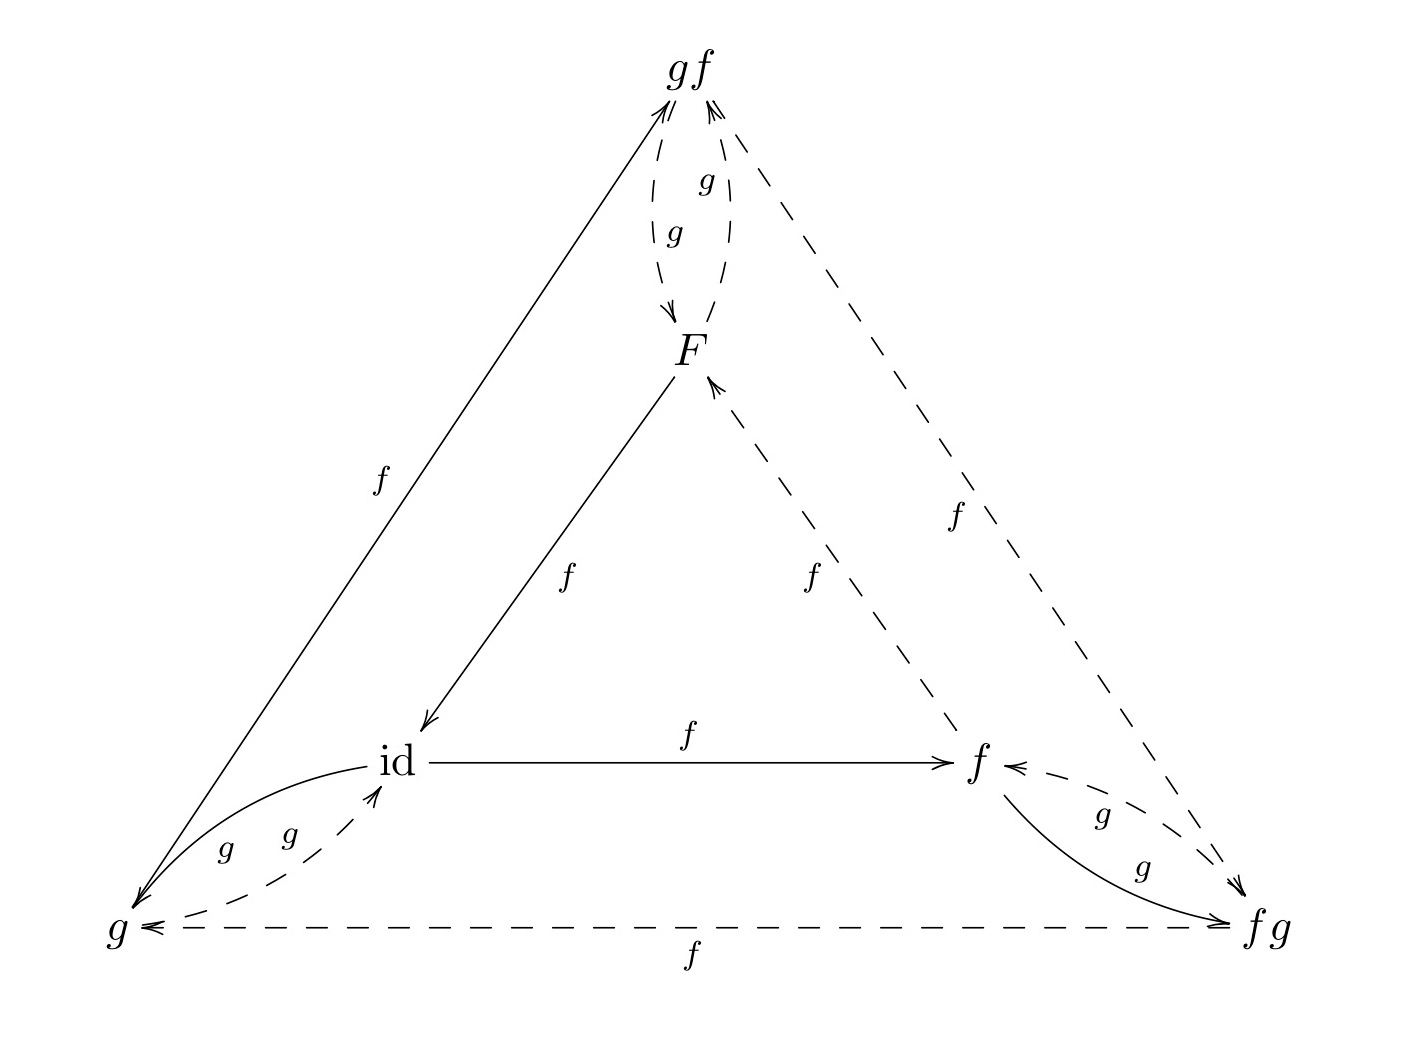
\includegraphics{./graphics/cayley-s3.jpg}}} Applying $R = \tau = (fg)^2$ at $x = f$ gives the cycle (top right\texttt{\symbol{45}}hand quadrilateral): 
\[ f \stackrel{f}{\longrightarrow} F \stackrel{g}{\longrightarrow} gf
\stackrel{f}{\longrightarrow} fg \stackrel{g}{\longrightarrow} f\ . \]
 Each of these edges has a non\texttt{\symbol{45}}trivial logged rewrite,
particularly the third edge where $gff \to gF \to fg$. Combining this log information we obtain: 
\[ [\tau,F]\,f ~=~ f.\tau ~=~ [1,{\rm id}].[-3,f][2,FG].[1,G][-3,{\rm
id}][2,FGF].[2,F]\,f . \]
 Expanding $[1,{\rm id}][-3,f][2,FG][1,G][-3,{\rm id}][2,FGF][2,F][-3,F]$ gives 
\[ fff.FGFGFf.gfggFG.gfffG.GFGF.fgfggFGF.fggF.fGFGFF \]
 which cancels to the identity, as expected. Converting this back to the group
presentation, we obtain the fourth identity given in the introduction (\ref{sect-illustration}): 
\[ \iota_{(\tau,f)} ~=~ \rho\ (\tau^{-1})^f\ \sigma^{FG}\ \rho^G\ (\tau^{-1})\
\sigma^{FGF}\ \sigma^F\ (\tau^{-1})^F\, . \]
 

 The operation \texttt{IdentityRelatorSequences} returns a list which omits any duplicates or empty lists. For the \texttt{s3} example, all of the possible $5*3 = 15$ sequences are added to the root identities. The relator just constructed is
the last but one in this list. }

 
\begin{Verbatim}[commandchars=!@|,fontsize=\small,frame=single,label=Example]
  
  !gapprompt@gap>| !gapinput@ms3 := MonoidPresentationFpGroup( s3 );;|
  !gapprompt@gap>| !gapinput@fms3 := FreeGroupOfPresentation( ms3 );;|
  !gapprompt@gap>| !gapinput@genfms3 := GeneratorsOfGroup(fms3 );;|
  !gapprompt@gap>| !gapinput@s3labs := ["f","g","F","G"];; |
  !gapprompt@gap>| !gapinput@SetMonoidPresentationLabels( ms3, s3labs );; |
  !gapprompt@gap>| !gapinput@idss3 := IdentityRelatorSequences( s3 );;          |
  !gapprompt@gap>| !gapinput@lenidss3 := Length( idss3 );                                   |
  17
  !gapprompt@gap>| !gapinput@List( idss3, L -> Length(L) );|
  [ 2, 2, 2, 2, 2, 2, 2, 2, 2, 2, 2, 2, 4, 4, 6, 8, 8 ]
  !gapprompt@gap>| !gapinput@ for i in [1..Length(idss3)] do                     |
  !gapprompt@>| !gapinput@      PrintLnUsingLabels( idss3[i], genfms3, s3labs );|
  !gapprompt@>| !gapinput@    od;|
  [ [ -3, id ], [ 3, f*g ] ]
  [ [ -3, id ], [ 3, G*F ] ]
  [ [ -2, id ], [ 2, g ] ]
  [ [ -2, id ], [ 2, G ] ]
  [ [ -1, id ], [ 1, f ] ]
  [ [ -1, id ], [ 1, F ] ]
  [ [ 1, id ], [ -1, f ] ]
  [ [ 1, id ], [ -1, F ] ]
  [ [ 1, G ], [ -1, F*G ] ]
  [ [ 2, id ], [ -2, G ] ]
  [ [ 2, F ], [ -2, G*F ] ]
  [ [ 3, f ], [ -3, G ] ]
  [ [ -3, f ], [ 2, F*G ], [ 3, f ], [ -2, f ] ]
  [ [ -2, F*G*F ], [ 3, id ], [ 2, id ], [ -3, G*F ] ]
  [ [ -2, F*G*F ], [ 3, id ], [ 1, G ], [ -3, id ], [ 2, F*G*F ], 
  [ -1, G*F ] ]
  [ [ 1, id ], [ -3, f ], [ 2, F*G ], [ 1, G ], [ -3, id ], 
  [ 2, F*G*F ], [ 2, F ], [ -3, F ] ]
  [ [ 1, G ], [ -3, id ], [ 2, F*G*F ], [ 2, F ], [ 1, id ], 
  [ -3, f ], [ 2, F*G ], [ -3, F*G ] ]
  
\end{Verbatim}
 

\subsection{\textcolor{Chapter }{LogSequenceLessThan}}
\logpage{[ 6, 1, 3 ]}\nobreak
\label{seq-less-than}
\hyperdef{L}{X7D9664267BC57E09}{}
{\noindent\textcolor{FuncColor}{$\triangleright$\enspace\texttt{LogSequenceLessThan({\mdseries\slshape J, K})\index{LogSequenceLessThan@\texttt{LogSequenceLessThan}}
\label{LogSequenceLessThan}
}\hfill{\scriptsize (operation)}}\\


 This is an operation used to sort lists of identity sequences. First the
lengths of sequences \texttt{J, K} are compared. If the lengths are equal then the sequences are compared as
lists. The list \texttt{idss3} is sorted using this function. 

 }

 
\begin{Verbatim}[commandchars=!@|,fontsize=\small,frame=single,label=Example]
  
  !gapprompt@gap>| !gapinput@LogSequenceLessThan( idss3[7], idss3[8] ); |
  true
  
\end{Verbatim}
 

\subsection{\textcolor{Chapter }{ExpandLogSequence}}
\logpage{[ 6, 1, 4 ]}\nobreak
\label{expand-log-seq}
\hyperdef{L}{X84E1E018809BE464}{}
{\noindent\textcolor{FuncColor}{$\triangleright$\enspace\texttt{ExpandLogSequence({\mdseries\slshape mG, L})\index{ExpandLogSequence@\texttt{ExpandLogSequence}}
\label{ExpandLogSequence}
}\hfill{\scriptsize (operation)}}\\


 This operation takes a log sequence $L$, writes each term as a conjugate of a relator, takes the product of all of
these, and then cancels consecutive inverse generators to return a word in the
free group of the presentation. This is precisely what we did by hand with $\iota_{(\tau,f)}$ on the previous page. If the sequence is an identity sequence the identity
element should be returned, so this provides a useful check. 

 }

 
\begin{Verbatim}[commandchars=!@|,fontsize=\small,frame=single,label=Example]
  
  !gapprompt@gap>| !gapinput@ExpandLogSequence( ms3, idss3[17] );|
  <identity ...>
  
\end{Verbatim}
 }

 
\section{\textcolor{Chapter }{Identities for $S_3$}}\label{sect-s3}
\logpage{[ 6, 2, 0 ]}
\hyperdef{L}{X79EE179E7AD81F44}{}
{
  We now return to the example considered in section \ref{sect-illustration}. In the previous section we have constructed $17$ identity sequences, and we now wish to reduce this number to find a minimal
set. 

\subsection{\textcolor{Chapter }{ReduceLogSequences}}
\logpage{[ 6, 2, 1 ]}\nobreak
\label{reduce-seq}
\hyperdef{L}{X8064D8CE783CB70A}{}
{\noindent\textcolor{FuncColor}{$\triangleright$\enspace\texttt{ReduceLogSequences({\mdseries\slshape G, ids})\index{ReduceLogSequences@\texttt{ReduceLogSequences}}
\label{ReduceLogSequences}
}\hfill{\scriptsize (operation)}}\\


 This operation applies a collection of operations, which will be described in
the following section, to reduce the list \texttt{idss3} from $17$ to $5$ identities. 

 }

 
\begin{Verbatim}[commandchars=!@|,fontsize=\small,frame=single,label=Example]
  
  !gapprompt@gap>| !gapinput@ridss3 := ReduceLogSequences( s3, idss3 );;|
  !gapprompt@gap>| !gapinput@lenridss3 := Length( ridss3 );                                   |
  5
  !gapprompt@gap>| !gapinput@for i in [1..lenridss3] do                                |
  !gapprompt@>| !gapinput@       PrintLnUsingLabels( ridss3[i], genfms3, s3labs );   |
  !gapprompt@>| !gapinput@   od;|
  [ [ -3, id ], [ 3, f*g ] ]
  [ [ -2, id ], [ 2, g ] ]
  [ [ -1, id ], [ 1, f ] ]
  [ [ 1, id ], [ -3, f ], [ 2, F*G ], [ 1, G ], [ -3, id ], 
  [ 2, F*G*F ], [ 2, F ], [ -3, F ] ]
  [ [ 1, id ], [ -3, g ], [ 2, F*G*F*g ], [ 2, F*g ], [ 1, g ], 
  [ -3, id ], [ 2, F ], [ -3, F ] ]
  
\end{Verbatim}
 We wish to show that the fifth of these identities is a combination of the
first four. Recall that the fourth identity was obtained by applying $R = \tau = (fg)^2$ at $x = f$. The fifth comes from applying $R = \tau$ at $x = gf$, so this is the same cycle but with a different start point. 

\subsection{\textcolor{Chapter }{ConjugateByWordLogSequence}}
\logpage{[ 6, 2, 2 ]}\nobreak
\label{conj-log-seq}
\hyperdef{L}{X82CCDCDF7BE58F35}{}
{\noindent\textcolor{FuncColor}{$\triangleright$\enspace\texttt{ConjugateByWordLogSequence({\mdseries\slshape mG, K, w})\index{ConjugateByWordLogSequence@\texttt{ConjugateByWordLogSequence}}
\label{ConjugateByWordLogSequence}
}\hfill{\scriptsize (operation)}}\\


 This operation conjugates every term in a log sequence by a word in the
generators. In the example we conjugate the fifth identity by $G$ to obtain \texttt{K5}. It then becomes apparent that the fourth identity \texttt{K4} has the form \texttt{[ A, B, [ \texttt{\symbol{45}}3, F ] ]} while \texttt{K5} has the form \texttt{[ B, A, [ \texttt{\symbol{45}}3, FG ] ]}, where the \texttt{F} and the \texttt{GF} are the inverses of the vertices where the cycle starts. 

 }

 
\begin{Verbatim}[commandchars=!@|,fontsize=\small,frame=single,label=Example]
  
  !gapprompt@gap>| !gapinput@K4 := ShallowCopy( ridss3[4] );; |
  !gapprompt@gap>| !gapinput@PrintLnUsingLabels( K4, genfms3, s3labs ); |
  [ [ 1, id ], [ -3, f ], [ 2, F*G ], [ 1, G ], [ -3, id ], 
  [ 2, F*G*F ], [ 2, F ], [ -3, F ] ]
  !gapprompt@gap>| !gapinput@L5 := ShallowCopy( ridss3[5] );; |
  !gapprompt@gap>| !gapinput@K5 := ConjugateByWordLogSequence( ms3, L5, genfms3[4] );; |
  !gapprompt@gap>| !gapinput@PrintLnUsingLabels( K5, genfms3, s3labs ); |
  [ [ 1, G ], [ -3, id ], [ 2, F*G*F ], [ 2, F ], [ 1, id ], 
  [ -3, f ], [ 2, F*G ], [ -3, F*G ] ]
  !gapprompt@gap>| !gapinput@A := K4{[1..3]};;              |
  !gapprompt@gap>| !gapinput@PrintLnUsingLabels( A, genfms3, s3labs ); |
  [ [ 1, id ], [ -3, f ], [ 2, F*G ] ]
  !gapprompt@gap>| !gapinput@B := K4{[4..7]};;              |
  !gapprompt@gap>| !gapinput@PrintLnUsingLabels( B, genfms3, s3labs ); |
  [ [ 1, G ], [ -3, id ], [ 2, F*G*F ], [ 2, F ] ]
  !gapprompt@gap>| !gapinput@PositionSublist( K5, A ); |
  5
  !gapprompt@gap>| !gapinput@PositionSublist( K5, B ); |
  1
  
\end{Verbatim}
 

\subsection{\textcolor{Chapter }{ChangeStartLogSequence}}
\logpage{[ 6, 2, 3 ]}\nobreak
\label{change-start}
\hyperdef{L}{X8220EF3585706C00}{}
{\noindent\textcolor{FuncColor}{$\triangleright$\enspace\texttt{ChangeStartLogSequence({\mdseries\slshape mon, K, p})\index{ChangeStartLogSequence@\texttt{ChangeStartLogSequence}}
\label{ChangeStartLogSequence}
}\hfill{\scriptsize (operation)}}\\


 

 The start point of an identity log sequence can be chosen at random (since
every conjugate of an identity is that identity). This operation permutes a
given sequence $K$ so as to start at the $p$\texttt{\symbol{45}}th position. 

 In our example we wish to show that \texttt{K4} and \texttt{K5} are equivalent up to root identities. To do this we first replace \texttt{K4} by \texttt{J4 = [ B, [ \texttt{\symbol{45}}3, F ], A ]}. 

 }

 
\begin{Verbatim}[commandchars=!@|,fontsize=\small,frame=single,label=Example]
  
  !gapprompt@gap>| !gapinput@J4 := ChangeStartLogSequence( ms3, K4, 4 );;|
  !gapprompt@gap>| !gapinput@PrintLnUsingLabels( J4, genfms3, s3labs ); |
  [ [ 1, G ], [ -3, id ], [ 2, F*G*F ], [ 2, F ], [ -3, F ], 
  [ 1, id ], [ -3, f ], [ 2, F*G ] ]
  
\end{Verbatim}
 

\subsection{\textcolor{Chapter }{InverseLogSequence}}
\logpage{[ 6, 2, 4 ]}\nobreak
\label{inv-log-seq}
\hyperdef{L}{X7E3DACB581C67E3C}{}
{\noindent\textcolor{FuncColor}{$\triangleright$\enspace\texttt{InverseLogSequence({\mdseries\slshape K})\index{InverseLogSequence@\texttt{InverseLogSequence}}
\label{InverseLogSequence}
}\hfill{\scriptsize (operation)}}\\


 

 To invert a log sequence we reverse the order of the terms and replace each \texttt{[m,w]} by \texttt{[\texttt{\symbol{45}}m,w]}. 

 We continue our example by replacing \texttt{J4} by its inverse. 

 }

 
\begin{Verbatim}[commandchars=!@|,fontsize=\small,frame=single,label=Example]
  
  !gapprompt@gap>| !gapinput@I4 := InverseLogSequence( J4 );; |
  !gapprompt@gap>| !gapinput@PrintLnUsingLabels( I4, genfms3, s3labs ); |
  [ [ -2, F*G ], [ 3, f ], [ -1, id ], [ 3, F ], [ -2, F ], [ -2, F*G*F ], 
  [ 3, id ], [ -1, G ] ]
  
\end{Verbatim}
 

\subsection{\textcolor{Chapter }{CancelImmediateInversesLogSequence}}
\logpage{[ 6, 2, 5 ]}\nobreak
\label{cancel-inverses}
\hyperdef{L}{X8325D1257B791ABC}{}
{\noindent\textcolor{FuncColor}{$\triangleright$\enspace\texttt{CancelImmediateInversesLogSequence({\mdseries\slshape K})\index{CancelImmediateInversesLogSequence@\texttt{CancelImmediateInversesLogSequence}}
\label{CancelImmediateInversesLogSequence}
}\hfill{\scriptsize (attribute)}}\\
\noindent\textcolor{FuncColor}{$\triangleright$\enspace\texttt{CancelInversesLogSequence({\mdseries\slshape mG, K})\index{CancelInversesLogSequence@\texttt{CancelInversesLogSequence}}
\label{CancelInversesLogSequence}
}\hfill{\scriptsize (operation)}}\\


 Concatenating \texttt{I4} and \texttt{K5}, we get \texttt{[ A\texttt{\symbol{94}}\texttt{\symbol{45}}1, [ 3, F ],
B\texttt{\symbol{94}}\texttt{\symbol{45}}1, B, A, [ \texttt{\symbol{45}}3, FG
] ]}, with length $16$. Cancelling immediate inverses removes the \texttt{[ B\texttt{\symbol{94}}\texttt{\symbol{45}}1, B ]}. Cancelling inverses gets rid of the terms \texttt{A\texttt{\symbol{94}}\texttt{\symbol{45}}1} and \texttt{A}, converting \texttt{[ 3, F ]} into \texttt{[ 3, fgFG ] = [ 3, FG ]}. Conjugating with \texttt{gf} produces the third root identity \texttt{[ [ 3, fg ], [ \texttt{\symbol{45}}3, id ] ]}, which then cancels. 

 }

 
\begin{Verbatim}[commandchars=!@|,fontsize=\small,frame=single,label=Example]
  
  !gapprompt@gap>| !gapinput@I4K5 := Concatenation( I4, K5 );; |
  !gapprompt@gap>| !gapinput@C1 := CancelImmediateInversesLogSequence( I4K5 );; |
  !gapprompt@gap>| !gapinput@PrintLnUsingLabels( C1, genfms3, s3labs ); |
  [ [ -2, F*G ], [ 3, f ], [ -1, id ], [ 3, F ], [ 1, id ], 
  [ -3, f ], [ 2, F*G ], [ -3, F*G ] ]
  !gapprompt@gap>| !gapinput@C2 := CancelInversesLogSequence( ms3, C1 ); |
  [ ]
  
\end{Verbatim}
 }

 
\section{\textcolor{Chapter }{Reducing identities}}\label{sect-reducing}
\logpage{[ 6, 3, 0 ]}
\hyperdef{L}{X82CE16C9788F883A}{}
{
  In this section we list some further operations which may be used to simplify
the list of identities returned by \texttt{IdentityRelatorSequences}. We will use our $Q_8$ presentation in the examples. 

 
\begin{Verbatim}[commandchars=!@|,fontsize=\small,frame=single,label=Example]
  
  !gapprompt@gap>| !gapinput@mq8 := MonoidPresentationFpGroup( q8 );;|
  !gapprompt@gap>| !gapinput@fmq8 := FreeGroupOfPresentation( mq8 );;|
  !gapprompt@gap>| !gapinput@genfmq8 := GeneratorsOfGroup(fmq8 );;|
  !gapprompt@gap>| !gapinput@q8labs := ["a","b","A","B"];; |
  !gapprompt@gap>| !gapinput@SetMonoidPresentationLabels( mq8, q8labs );; |
  !gapprompt@gap>| !gapinput@idsq8 := IdentityRelatorSequences( q8 );;          |
  !gapprompt@gap>| !gapinput@lenidsq8 := Length( idsq8 );                                   |
  28
  !gapprompt@gap>| !gapinput@List( idsq8, L -> Length(L) );|
  [ 2, 2, 2, 2, 2, 2, 2, 4, 4, 4, 4, 4, 4, 4, 4, 4, 5, 5, 5, 6, 6, 7, 8, 8, 8, 
    9, 10, 10 ]
  
\end{Verbatim}
 

\subsection{\textcolor{Chapter }{LogSequenceRewriteRules}}
\logpage{[ 6, 3, 1 ]}\nobreak
\label{root-rules}
\hyperdef{L}{X80F769D9796954FC}{}
{\noindent\textcolor{FuncColor}{$\triangleright$\enspace\texttt{LogSequenceRewriteRules({\mdseries\slshape mG})\index{LogSequenceRewriteRules@\texttt{LogSequenceRewriteRules}}
\label{LogSequenceRewriteRules}
}\hfill{\scriptsize (attribute)}}\\


 The root identity $R^{-1}R^w$ may be converted into the rewrite rule $R^w \to R$. 

 }

 
\begin{Verbatim}[commandchars=!@|,fontsize=\small,frame=single,label=Example]
  
  !gapprompt@gap>| !gapinput@rulesq8 := LogSequenceRewriteRules( mq8 );;|
  !gapprompt@gap>| !gapinput@for i in [1..8] do |
  !gapprompt@>| !gapinput@       PrintLnUsingLabels( rulesq8[i], genfmq8, q8labs );|
  !gapprompt@>| !gapinput@   od;|
  [ [ 1, a ], [ 1, id ] ]
  [ [ -1, a ], [ -1, id ] ]
  [ [ 1, A ], [ 1, id ] ]
  [ [ -1, A ], [ -1, id ] ]
  [ [ 2, b ], [ 2, id ] ]
  [ [ -2, b ], [ -2, id ] ]
  [ [ 2, B ], [ 2, id ] ]
  [ [ -2, B ], [ -2, id ] ]
  [ [ 3, a*b*a*B ], [ 3, id ] ]
  [ [ 3, b*A*B*A ], [ 3, id ] ]
  [ [ -3, a*b*a*B ], [ -3, id ] ]
  [ [ -3, b*A*B*A ], [ -3, id ] ]
  [ [ 4, a^2*b^2 ], [ 4, id ] ]
  [ [ 4, B^2*A^2 ], [ 4, id ] ]
  [ [ -4, a^2*b^2 ], [ -4, id ] ]
  [ [ -4, B^2*A^2 ], [ -4, id ] ]
  
\end{Verbatim}
 

\subsection{\textcolor{Chapter }{OnePassReduceLogSequence}}
\logpage{[ 6, 3, 2 ]}\nobreak
\label{one-pass-red-seq}
\hyperdef{L}{X82F66A16877FCDFE}{}
{\noindent\textcolor{FuncColor}{$\triangleright$\enspace\texttt{OnePassReduceLogSequence({\mdseries\slshape J, rules})\index{OnePassReduceLogSequence@\texttt{OnePassReduceLogSequence}}
\label{OnePassReduceLogSequence}
}\hfill{\scriptsize (operation)}}\\


 The rewrite rules returned by \texttt{LogSequenceRewriteRules} may be used to simplify other identity sequences. In the example the fourth
rule $(q^{-1})^A \to q^{-1}$, applied twice, reduces $(q^{-1})^{A^2}$ to $q^{-1}$. 

 }

 
\begin{Verbatim}[commandchars=!@|,fontsize=\small,frame=single,label=Example]
  
  !gapprompt@gap>| !gapinput@J7 := idsq8[7];|
  [ [ 1, <identity ...> ], [ -1, q8_M3^2 ] ]
  !gapprompt@gap>| !gapinput@OnePassReduceLogSequence( J7, rulesq8 );|
  [ [ 1, <identity ...> ], [ -1, <identity ...> ] ]
  
\end{Verbatim}
 The operation \texttt{ReduceLogSequences}, described in subsection \ref{reduce-seq}, applied to the list \texttt{idsq8} reduces the $28$ identities to $15$. 

 
\begin{Verbatim}[commandchars=!@|,fontsize=\small,frame=single,label=Example]
  
  !gapprompt@gap>| !gapinput@ridsq8 := ReduceLogSequences( q8, idsq8 );;|
  !gapprompt@gap>| !gapinput@lenrids := Length( ridsq8 );                                   |
  15
  !gapprompt@gap>| !gapinput@for i in [1..lenrids] do                                |
  !gapprompt@>| !gapinput@       PrintLnUsingLabels( ridsq8[i], genfmq8, q8labs );   |
  !gapprompt@>| !gapinput@   od;|
  [ [ -2, id ], [ 2, b ] ]
  [ [ -1, id ], [ 1, a ] ]
  [ [ -4, id ], [ 2, A^2 ], [ 1, id ], [ -4, a^2 ] ]
  [ [ -4, id ], [ 3, A ], [ 4, a ], [ -3, b ] ]
  [ [ 1, id ], [ -4, id ], [ 2, A^2 ], [ -4, A^2 ] ]
  [ [ -4, id ], [ 3, A ], [ 3, id ], [ 2, id ], [ -4, b ] ]
  [ [ -3, id ], [ 4, B*A ], [ -4, A ], [ 1, id ], [ -3, a ] ]
  [ [ -3, id ], [ 4, B*A ], [ -4, A^2 ], [ 1, id ], [ -3, B ] ]
  [ [ -4, id ], [ 3, A ], [ -4, A ], [ 2, A^3 ], [ 1, id ], 
  [ -3, b ] ]
  [ [ -4, id ], [ 4, B*A^2 ], [ -4, A^2 ], [ 1, id ], [ 2, id ], 
  [ -4, b ] ]
  [ [ -3, id ], [ 4, B*A ], [ -4, A ], [ 3, A^2 ], [ 4, id ], 
  [ -4, B ] ]
  [ [ -4, id ], [ 3, A ], [ 4, B*A ], [ -4, A ], [ 1, id ], 
  [ -3, a ], [ 4, B ], [ -1, b ] ]
  [ [ -3, id ], [ 4, B*A ], [ -4, A ], [ 3, A^2 ], [ 4, B*A^2 ], 
  [ -4, A^2 ], [ 1, id ], [ -1, B ] ]
  [ [ 4, id ], [ -4, b ], [ 1, b ], [ -3, a^2*b ], [ 4, B*a*b ], 
  [ -4, a*b ], [ 3, b ], [ -1, id ] ]
  [ [ -3, id ], [ 4, B*A ], [ -4, A ], [ 1, id ], [ -4, a ], 
  [ 2, A ], [ 1, id ], [ -4, a^2 ], [ -3, B ] ] 
  
\end{Verbatim}
 We now demonstrate that this list may be reduced further. 

\subsection{\textcolor{Chapter }{MoveRightLogSequence}}
\logpage{[ 6, 3, 3 ]}\nobreak
\label{move-left-right}
\hyperdef{L}{X85814EFA81FE864F}{}
{\noindent\textcolor{FuncColor}{$\triangleright$\enspace\texttt{MoveRightLogSequence({\mdseries\slshape mG, J, L, q})\index{MoveRightLogSequence@\texttt{MoveRightLogSequence}}
\label{MoveRightLogSequence}
}\hfill{\scriptsize (operation)}}\\
\noindent\textcolor{FuncColor}{$\triangleright$\enspace\texttt{MoveLeftLogSequence({\mdseries\slshape mG, J, L, q})\index{MoveLeftLogSequence@\texttt{MoveLeftLogSequence}}
\label{MoveLeftLogSequence}
}\hfill{\scriptsize (operation)}}\\
\noindent\textcolor{FuncColor}{$\triangleright$\enspace\texttt{SwapLogSequence({\mdseries\slshape mG, J, p, q})\index{SwapLogSequence@\texttt{SwapLogSequence}}
\label{SwapLogSequence}
}\hfill{\scriptsize (operation)}}\\


 The terms in an identity sequence may be interchanged because 
\[ R^w Q^v ~=~ Q^v R^{wQ^v} ~=~ Q^{v(R^w)^{-1}} R^w. \]
 In the first two of these three operations \texttt{L =} $[p..r]$ is a range specifying a sublist \texttt{K=J\texttt{\symbol{123}}[p..r]\texttt{\symbol{125}}} of \texttt{J}, and $l$ is the length of \texttt{J}. The operation \texttt{MoveRightLogSequence(mG,J,L,q)}, with $0$ {\textless} $p$ {\textless} $q$ and $q+r \leq p+l$, moves sublist \texttt{K} to the $q$\texttt{\symbol{45}}th position, conjugating entries in $J\{[p+1 \ldots q]\}$ and moving them all to the left. 

 Similarly \texttt{MoveLeftLogSequence(mG,J,L,q)}, with $0$ {\textless} $q$ {\textless} $p$ nd $r \leq l$, moves sublist \texttt{K} to the $q$\texttt{\symbol{45}}th position, conjugating entries in $J\{[q \ldots p-1]\}$ and moving them all to the right. 

 The operation \texttt{SwapLogSequence(mG,J,p,q)} with $p$ {\textless} $q$ swaps a pair of terms in a sequence \texttt{J} by calling the two previous commands. 

 In all three operations the procedure is completed by a call to \texttt{OnePassReduceLogSequence}. 

 In the example the third identity is converted into the fifth by moving the
third term one place right and then changing the start position, so it may be
omitted. 

 }

 
\begin{Verbatim}[commandchars=!@|,fontsize=\small,frame=single,label=Example]
  
  !gapprompt@gap>| !gapinput@J3 := ShallowCopy( ridsq8[3] );;                            |
  !gapprompt@gap>| !gapinput@PrintLnUsingLabels( J3, genfmq8, q8labs );   |
  [ [ -4, id ], [ 2, A^2 ], [ 1, id ], [ -4, a^2 ] ]
  !gapprompt@gap>| !gapinput@K3 := MoveRightLogSequence( mq8, J3, [3], 4 );;|
  !gapprompt@gap>| !gapinput@PrintLnUsingLabels( K3, genfmq8, q8labs );    |
  [ [ -4, id ], [ 2, A^2 ], [ -4, A^2 ], [ 1, id ] ]
  !gapprompt@gap>| !gapinput@J5 := ShallowCopy( ridsq8[5] );; |
  !gapprompt@gap>| !gapinput@PrintLnUsingLabels( J5, genfmq8, q8labs );|
  [ [ 1, id ], [ -4, id ], [ 2, A^2 ], [ -4, A^2 ] ]
  !gapprompt@gap>| !gapinput@J5 = ChangeStartLogSequence( mq8, K3, 4 );|
  true
  
\end{Verbatim}
 

\subsection{\textcolor{Chapter }{SubstituteLogSubsequence}}
\logpage{[ 6, 3, 4 ]}\nobreak
\label{subs-log-seq}
\hyperdef{L}{X7EE8CE5E79598779}{}
{\noindent\textcolor{FuncColor}{$\triangleright$\enspace\texttt{SubstituteLogSubsequence({\mdseries\slshape mG, K, J1, J2})\index{SubstituteLogSubsequence@\texttt{SubstituteLogSubsequence}}
\label{SubstituteLogSubsequence}
}\hfill{\scriptsize (operation)}}\\


 If we move the second term in \texttt{J5} to the right, we find that sublist \texttt{U = [[1,id],[2,id]]} is equal to \texttt{V = [[4,A\texttt{\symbol{94}}2],[4,id]]}, with both expanding to $a^4b^4$. 

 Now \texttt{U} appears in the tenth identity, and if we replace it with \texttt{V} and then cancel, we obtain the empty list. So the tenth identity may be
omitted. }

 
\begin{Verbatim}[commandchars=!@|,fontsize=\small,frame=single,label=Example]
  
  !gapprompt@gap>| !gapinput@K5 := MoveRightLogSequence( mq8, J5, [2], 3 );;|
  !gapprompt@gap>| !gapinput@PrintLnUsingLabels( K5, genfmq8, q8labs );       |
  [ [ 1, id ], [ 2, id ], [ -4, id ], [ -4, A^2 ] ]
  !gapprompt@gap>| !gapinput@K5a := K5{[1..2]};; |
  !gapprompt@gap>| !gapinput@K5b := InverseLogSequence( K5{[3..4]} );;|
  !gapprompt@gap>| !gapinput@K5a;K5b;|
  [ [ 1, <identity ...> ], [ 2, <identity ...> ] ]
  [ [ 4, q8_M3^2 ], [ 4, <identity ...> ] ]
  !gapprompt@gap>| !gapinput@J10 := ShallowCopy( ridsq8[10] );;|
  !gapprompt@gap>| !gapinput@PrintLnUsingLabels( J10, genfmq8, q8labs );|
  [ [ -4, id ], [ 4, B*A^2 ], [ -4, A^2 ], [ 1, id ], [ 2, id ], 
  [ -4, b ] ]
  !gapprompt@gap>| !gapinput@K10 := SubstituteLogSubsequence( mq8, J10, K5a, K5b );;|
  !gapprompt@gap>| !gapinput@PrintLnUsingLabels( K10, genfmq8, q8labs );            |
  [ [ -4, id ], [ 4, B*A^2 ], [ -4, A^2 ], [ 4, A^2 ], [ 4, id ], 
  [ -4, b ] ]
  !gapprompt@gap>| !gapinput@CancelInversesLogSequence( mq8, K10 );|
  [  ]
  
\end{Verbatim}
 Similarly, we may reduce the ninth identity. Initially, \texttt{U} does not appear as a sublist of \texttt{J9}. Swapping the fourth and fifth terms and conjugating by $A$ produces \texttt{U}, which is then replaced by \texttt{V}. After a cancellation, we obtain a conjugate of the fourth identity. 

 
\begin{Verbatim}[commandchars=!@|,fontsize=\small,frame=single,label=Example]
  
  !gapprompt@gap>| !gapinput@J9 := ShallowCopy( ridsq8[9] );; |
  !gapprompt@gap>| !gapinput@PrintLnUsingLabels( J9, genfmq8, q8labs );            |
  [ [ -4, id ], [ 3, A ], [ -4, A ], [ 2, A^3 ], [ 1, id ], 
  [ -3, b ] ]
  !gapprompt@gap>| !gapinput@K9 := MoveLeftLogSequence( mq8, J9, [5], 4 );; |
  !gapprompt@gap>| !gapinput@PrintLnUsingLabels( K9, genfmq8, q8labs );            |
  [ [ -4, id ], [ 3, A ], [ -4, A ], [ 1, id ], [ 2, a ], [ -3, b ] ]
  !gapprompt@gap>| !gapinput@L9 := ConjugateByWordLogSequence( mq8, K9, genfmq8[3] );;|
  !gapprompt@gap>| !gapinput@PrintLnUsingLabels( L9, genfmq8, q8labs );            |
  [ [ -4, A ], [ 3, A^2 ], [ -4, A^2 ], [ 1, id ], [ 2, id ], 
  [ -3, b*A ] ]
  !gapprompt@gap>| !gapinput@M9 := SubstituteLogSubsequence( mq8, L9, K5a, K5b);;|
  !gapprompt@gap>| !gapinput@PrintLnUsingLabels( M9, genfmq8, q8labs );            |
  [ [ -4, A ], [ 3, A^2 ], [ -4, A^2 ], [ 4, A^2 ], [ 4, id ], 
  [ -3, b*A ] ]
  !gapprompt@gap>| !gapinput@N9 := CancelInversesLogSequence( mq8, M9 );;|
  !gapprompt@gap>| !gapinput@PrintLnUsingLabels( N9, genfmq8, q8labs );            |
  [ [ -4, A ], [ 3, A^2 ], [ 4, id ], [ -3, b*A ] ]
  !gapprompt@gap>| !gapinput@P9 := ConjugateByWordLogSequence( mq8, N9, genfmq8[1] );;|
  !gapprompt@gap>| !gapinput@PrintLnUsingLabels( P9, genfmq8, q8labs );            |
  [ [ -4, id ], [ 3, A ], [ 4, a ], [ -3, b ] ]
  !gapprompt@gap>| !gapinput@P9 = ridsq8[4];|
  true
  
\end{Verbatim}
 We will not, for now, attempt to reduce the list of identities further. }

 
\section{\textcolor{Chapter }{The original approach}}\label{sect-original}
\logpage{[ 6, 4, 0 ]}
\hyperdef{L}{X7D428F9B8054F5FB}{}
{
  This section describes the approach used from the earliest versions of \textsf{IdRel} up to version 2.38 in 2017. For version 2.39 the methods were revised so as to
produce some data for infinite groups. This experimental work is described in
later sections. 

\subsection{\textcolor{Chapter }{IdentitiesAmongRelators}}
\logpage{[ 6, 4, 1 ]}\nobreak
\hyperdef{L}{X7FD998C87BF9AAC9}{}
{\noindent\textcolor{FuncColor}{$\triangleright$\enspace\texttt{IdentitiesAmongRelators({\mdseries\slshape grp})\index{IdentitiesAmongRelators@\texttt{IdentitiesAmongRelators}}
\label{IdentitiesAmongRelators}
}\hfill{\scriptsize (attribute)}}\\


 

 It is \emph{not} guaranteed that a minimal set of identities is obtained. For \texttt{q8} a set of seven identities is returned, whereas a minimal set contains only
six. See Example 5.1 of \cite{HeWe1} for further details. 

 Why \texttt{idrelq8} in the following example is shorter than \texttt{ridsq8} above remains to be investigated! 

 }

 
\begin{Verbatim}[commandchars=!@|,fontsize=\small,frame=single,label=Example]
  
  !gapprompt@gap>| !gapinput@idrelq8 := IdentitiesAmongRelators( q8 );;|
  !gapprompt@gap>| !gapinput@Length( idrelq8 );|
  14
  !gapprompt@gap>| !gapinput@for i in [1..14] do |
  !gapprompt@>| !gapinput@      PrintLnUsingLabels( idrelq8[i], genfmq8, q8labs ); |
  !gapprompt@>| !gapinput@   od; |
  [ [ -1, id ], [ 1, a ] ]
  [ [ -2, id ], [ 2, b ] ]
  [ [ -4, id ], [ 3, A ], [ 3, id ], [ 2, id ], [ -4, b ] ]
  [ [ -4, id ], [ 2, A^2 ], [ 1, id ], [ -4, a^2 ] ]
  [ [ 1, id ], [ -4, id ], [ 2, A^2 ], [ -4, A^2 ] ]
  [ [ -3, id ], [ 4, B*A ], [ -4, A ], [ 1, id ], [ -3, a ] ]
  [ [ -4, id ], [ 3, A ], [ 4, a ], [ -3, b ] ]
  [ [ -3, id ], [ 4, B*A ], [ -4, A^2 ], [ 1, id ], [ -3, B ] ]
  [ [ -4, id ], [ 4, B*A^2 ], [ -4, A^2 ], [ 1, id ], [ 2, id ], 
  [ -4, b ] ]
  [ [ -3, id ], [ 4, B*A ], [ -4, A ], [ 3, A^2 ], [ 4, id ], 
  [ -4, B ] ]
  [ [ -4, id ], [ 3, A ], [ -4, A ], [ 2, A^3 ], [ 1, id ], 
  [ -3, b ] ]
  [ [ -3, id ], [ 4, B*A ], [ -4, A ], [ 1, id ], [ -4, a ], 
  [ 2, A ], [ 1, id ], [ -4, a^2 ], [ -3, B ] ]
  [ [ -4, id ], [ 3, A ], [ 4, B*A ], [ -4, A ], [ 1, id ], 
  [ -3, a ], [ 4, B ], [ -1, b ] ]
  [ [ -3, id ], [ 4, B*A ], [ -4, A ], [ 3, A^2 ], [ 4, B*A^2 ], 
  [ -4, A^2 ], [ 1, id ], [ -1, B ] ]
  
\end{Verbatim}
 

\subsection{\textcolor{Chapter }{IdentityYSequences}}
\logpage{[ 6, 4, 2 ]}\nobreak
\hyperdef{L}{X78A94CB77B98ACAA}{}
{\noindent\textcolor{FuncColor}{$\triangleright$\enspace\texttt{IdentityYSequences({\mdseries\slshape grp})\index{IdentityYSequences@\texttt{IdentityYSequences}}
\label{IdentityYSequences}
}\hfill{\scriptsize (attribute)}}\\


 These identities are then transformed into module polynomials 
\[ \rho(a + ba) + \sigma({\rm id} + ab + ba) - \tau({\rm id} + a + A)\ , \]
 where the monoid elements are transformed into their normal forms. 

 The collection of saturated sets of these module polynomials is then reduced
as far as possible, and the minimal set obtained returned as the \texttt{IdentityYSequences} of the group. The group relator sequences corresponding to these module
polynomials form the \texttt{IdentitiesAmongRelators} for the group. 

 }

 
\begin{Verbatim}[commandchars=!@|,fontsize=\small,frame=single,label=Example]
  
  !gapprompt@gap>| !gapinput@idyseq8 := IdentityYSequences( q8 );; |
  !gapprompt@gap>| !gapinput@for y in idyseq8 do |
  !gapprompt@>| !gapinput@       PrintLnYSequence( y, genfmq8, q8labs, genq8R, q8Rlabs ); |
  !gapprompt@>| !gapinput@   od; |
  q8_Y2*(1*A), q^-1*(-1*A) + q*(1*id)) 
  q8_Y1*(1*B), r^-1*(-1*B) + r*(1*id)) 
  q8_Y6*(-1*id), r*(-1*id) + s*(-1*A + -1*id) + t^-1*(1*b + 1*id)) 
  q8_Y3*(-1*a), q*(-1*a) + r*(-1*A) + t^-1*(1*A + 1*a)) 
  q8_Y5*(-1*a), q*(-1*a) + r*(-1*A) + t^-1*(1*A + 1*a)) 
  q8_Y7*(1*a*b), q*(1*a*b) + s^-1*(-1*a*b + -1*B) + t^-1*(-1*b) + t*(1*id)) 
  q8_Y4*(1*A), s^-1*(-1*a*b) + s*(1*a^2) + t^-1*(-1*A) + t*(1*id)) 
  q8_Y8*(1*a*b), q*(1*a*b) + s^-1*(-1*a*b + -1*A) + t^-1*(-1*a*B) + t*(1*id)) 
  q8_Y10*(1*B), q*(1*B) + r*(1*B) + t^-1*(-1*B + -1*b + -1*id) + t*(1*id)) 
  q8_Y11*(1*b), s^-1*(-1*b) + s*(1*B) + t^-1*(-1*a*B + -1*id) + t*(1*b + 1*a)) 
  q8_Y9*(-1*a), q*(-1*a) + r*(-1*a^2) + s^-1*(1*a*B) + s*(-1*id) + t^-1*(1*a + 
  1*id)) 
  q8_Y15*(1*a*b), q*(2*a*b) + r*(1*b) + s^-1*(-1*a*b + -1*A) + t^-1*(-1*a*B + 
  -1*B + -1*b) + t*(1*id)) 
  q8_Y12*(1*b), q^-1*(-1*a^2) + q*(1*b) + s^-1*(-1*a*b) + s*(1*a*B) + t^-1*(
  -1*a*B + -1*b) + t*(1*a + 1*id)) 
  q8_Y13*(1*a*b), q^-1*(-1*A) + q*(1*a*b) + s^-1*(-1*a*b) + s*(1*a*B) + t^-1*(
  -1*a*B + -1*b) + t*(1*a + 1*id)) 
  
\end{Verbatim}
 }

 
\section{\textcolor{Chapter }{Partial lists of elements}}\label{sect-partial-elements}
\logpage{[ 6, 5, 0 ]}
\hyperdef{L}{X8448909D82CF6FE9}{}
{
  As we have seen, the procedure for obtaining identities involves applying each
relator at each element of the group. Since this will not terminate when the
group is infinite, we include an operation to construct words up to a given
length in the monoid representation of the group. 

\subsection{\textcolor{Chapter }{PartialElementsOfMonoidRepresentation}}
\logpage{[ 6, 5, 1 ]}\nobreak
\hyperdef{L}{X7FCEF03E7A57C331}{}
{\noindent\textcolor{FuncColor}{$\triangleright$\enspace\texttt{PartialElementsOfMonoidRepresentation({\mdseries\slshape G, len})\index{PartialElementsOfMonoidRepresentation@\texttt{Partial}\-\texttt{Elements}\-\texttt{Of}\-\texttt{Monoid}\-\texttt{Representation}}
\label{PartialElementsOfMonoidRepresentation}
}\hfill{\scriptsize (operation)}}\\


 As an example we take the group $\langle u,v,w ~|~ u^3, v^2, w^2, (uv)^2, (vw)^2\rangle$. 

 }

 
\begin{Verbatim}[commandchars=!@|,fontsize=\small,frame=single,label=Example]
  
  !gapprompt@gap>| !gapinput@F := FreeGroup(3);;|
  !gapprompt@gap>| !gapinput@u := F.1;;  v := F.2;;  w := F.3;;|
  !gapprompt@gap>| !gapinput@rels := [ u^3, v^2, w^2, (u*v)^2, (v*w)^2 ];;|
  !gapprompt@gap>| !gapinput@q0 := F/rels;;|
  !gapprompt@gap>| !gapinput@SetArrangementOfMonoidGenerators( q0, [1,-1,2,-2,3,-3] );|
  !gapprompt@gap>| !gapinput@SetName( q0, "q0" );|
  !gapprompt@gap>| !gapinput@mq0 := MonoidPresentationFpGroup( q0 );;|
  !gapprompt@gap>| !gapinput@fmq0 := FreeGroupOfPresentation( mq0 );;|
  !gapprompt@gap>| !gapinput@genfmq0 := GeneratorsOfGroup( fmq0 );;|
  !gapprompt@gap>| !gapinput@q0labs := ["u","U","v","V","w","W"];; |
  !gapprompt@gap>| !gapinput@SetMonoidPresentationLabels( mq0, q0labs );; |
  !gapprompt@gap>| !gapinput@lrws := LoggedRewritingSystemFpGroup( q0 );;|
  !gapprompt@gap>| !gapinput@pe1 := PartialElementsOfMonoidPresentation( q0, 1 );; |
  !gapprompt@gap>| !gapinput@PrintLnUsingLabels( pe1, genfmq0, q0labs ); |
  [ id, u, U, v, w ]
  !gapprompt@gap>| !gapinput@pe2 := PartialElementsOfMonoidPresentation( q0, 2 );;|
  !gapprompt@gap>| !gapinput@PrintLnUsingLabels( pe2, genfmq0, q0labs ); |
  [ id, u, U, v, w, u*v, u*w, U*v, U*w, v*w, w*u, w*U ]
  
\end{Verbatim}
 }

 }

 \def\bibname{References\logpage{[ "Bib", 0, 0 ]}
\hyperdef{L}{X7A6F98FD85F02BFE}{}
}

\bibliographystyle{alpha}
\bibliography{bib.xml}

\addcontentsline{toc}{chapter}{References}

\def\indexname{Index\logpage{[ "Ind", 0, 0 ]}
\hyperdef{L}{X83A0356F839C696F}{}
}

\cleardoublepage
\phantomsection
\addcontentsline{toc}{chapter}{Index}


\printindex

\immediate\write\pagenrlog{["Ind", 0, 0], \arabic{page},}
\newpage
\immediate\write\pagenrlog{["End"], \arabic{page}];}
\immediate\closeout\pagenrlog
\end{document}
